% -*- TeX-engine: xetex; eval: (auto-fill-mode 0); eval: (visual-line-mode 1); -*-
% Compile with XeLaTeX

%%%%%%%%%%%%%%%%%%%%%%%
% Option 1: Slides: (comment for handouts)   %
%%%%%%%%%%%%%%%%%%%%%%%

%\documentclass[slidestop,compress,mathserif,12pt,t,professionalfonts,xcolor=table]{beamer}

% solution stuff
%\newcommand{\solnMult}[1]{
%\only<1>{#1}
%\only<2->{\red{\textbf{#1}}}
%}
%\newcommand{\soln}[1]{\textit{#1}}

%%%%%%%%%%%%%%%%%%%%%%%%%%%%%%%
% Option 2: Handouts, without solutions (post before class)    %
%%%%%%%%%%%%%%%%%%%%%%%%%%%%%%%

 \documentclass[11pt,containsverbatim,handout,xcolor=xelatex,dvipsnames,table]{beamer}

 % handout layout
 \usepackage{pgfpages}
 \pgfpagesuselayout{4 on 1}[letterpaper,landscape,border shrink=5mm]

%% % solution stuff
 \newcommand{\solnMult}[1]{#1}
 \newcommand{\soln}[1]{}

%%%%%%%%%%%%%%%%%%%%%%%%%%%%%%%%%%%%
% Option 3: Handouts, with solutions (may post after class if need be)    %
%%%%%%%%%%%%%%%%%%%%%%%%%%%%%%%%%%%%

% \documentclass[11pt,containsverbatim,handout,xcolor=xelatex,dvipsnames,table]{beamer}

% % handout layout
% \usepackage{pgfpages}
% \pgfpagesuselayout{4 on 1}[letterpaper,landscape,border shrink=5mm]

% % solution stuff
% \newcommand{\solnMult}[1]{\red{\textbf{#1}}}
% \newcommand{\soln}[1]{\textit{#1}}

%%%%%%%%%%
% Load style file, defaults  %
%%%%%%%%%%

%%%%%%%%%%%%%%%%
% Themes
%%%%%%%%%%%%%%%%

% See http://deic.uab.es/~iblanes/beamer_gallery/ for mor options

% Style theme
\usetheme{Pittsburgh}

% Color theme
\usecolortheme{seahorse}

% Helvetica Neue Light for most text
\usepackage{fontspec}
\setsansfont{Helvetica Neue Light}

%%%%%%%%%%%%%%%%
% Packages
%%%%%%%%%%%%%%%%

\usepackage{geometry}
\usepackage{graphicx}
\usepackage{amssymb}
\usepackage{epstopdf}
\usepackage{amsmath}  	% this permits text in eqnarray among other benefits
\usepackage{url}		% produces hyperlinks
\usepackage[english]{babel}
\usepackage{colortbl}	% allows for color usage in tables
\usepackage{multirow}	% allows for rows that span multiple rows in tables
\usepackage{color}		% this package has a variety of color options
\usepackage{pgf}
\usepackage{calc}
\usepackage{ulem}
\usepackage{multicol}
\usepackage{textcomp}
\usepackage{listings}
\usepackage{changepage}
\usepackage{tikz}
\usetikzlibrary{trees}		% for probability trees
\usepackage{fancyvrb}	% for colored code chunks
\usepackage{nameref}

%%%%%%%%%%%%%%%%
% Remove navigation symbols
%%%%%%%%%%%%%%%%

\beamertemplatenavigationsymbolsempty
\hypersetup{pdfpagemode=UseNone} % don't show bookmarks on initial view

%%%%%%%%%%%%%%%%
% User defined colors
%%%%%%%%%%%%%%%%

% Pantone 2016 Spring colors
% https://atelierbram.github.io/c-tiles16/colorscheming/pantone-spring-2016-colortable.html
% update each semester or year

\xdefinecolor{custom_blue}{rgb}{0.01, 0.31, 0.52} % Snorkel Blue
\xdefinecolor{custom_darkBlue}{rgb}{0.20, 0.20, 0.39} % Reflecting Pond  
\xdefinecolor{custom_orange}{rgb}{0.96, 0.57, 0.42} % Cadmium Orange
\xdefinecolor{custom_green}{rgb}{0, 0.47, 0.52} % Biscay Bay
\xdefinecolor{custom_red}{rgb}{0.58, 0.32, 0.32} % Marsala

\xdefinecolor{custom_lightGray}{rgb}{0.78, 0.80, 0.80} % Glacier Gray
\xdefinecolor{custom_darkGray}{rgb}{0.35, 0.39, 0.43} % Stormy Weather

%%%%%%%%%%%%%%%%
% Template colors
%%%%%%%%%%%%%%%%

\setbeamercolor*{palette primary}{fg=white,bg= custom_blue}
\setbeamercolor*{palette secondary}{fg=black,bg= custom_blue!80!black}
\setbeamercolor*{palette tertiary}{fg=white,bg= custom_blue!80!black!80}
\setbeamercolor*{palette quaternary}{fg=white,bg= custom_blue}

\setbeamercolor{structure}{fg= custom_blue}
\setbeamercolor{frametitle}{bg= custom_blue!90}
\setbeamertemplate{blocks}[shadow=false]
\setbeamersize{text margin left=2em,text margin right=2em}

%%%%%%%%%%%%%%%%
% Styling fonts, bullets, etc.
%%%%%%%%%%%%%%%%

% title slide
\setbeamerfont{title}{size=\large,series=\bfseries}
\setbeamerfont{subtitle}{size=\large,series=\mdseries}
%\setbeamerfont{institute}{size=\large,series=\mdseries}

% color of alerted text
\setbeamercolor{alerted text}{fg=custom_orange}

% styling of itemize bullets
\setbeamercolor{item}{fg=custom_blue}
\setbeamertemplate{itemize item}{{{\small$\blacktriangleright$}}}
\setbeamercolor{subitem}{fg=custom_blue}
\setbeamertemplate{itemize subitem}{{\textendash}}
\setbeamerfont{itemize/enumerate subbody}{size=\footnotesize}
\setbeamerfont{itemize/enumerate subitem}{size=\footnotesize}

% styling of enumerate bullets
\setbeamertemplate{enumerate item}{\insertenumlabel.}
\setbeamerfont{enumerate item}{family={\fontspec{Helvetica Neue}}}
\setbeamerfont{enumerate subitem}{family={\fontspec{Helvetica Neue}}}
\setbeamerfont{enumerate subsubitem}{family={\fontspec{Helvetica Neue}}}

% make frame titles small to make room in the slide
\setbeamerfont{frametitle}{size=\small} 

% set Helvetica Neue font for frame and section titles
\setbeamerfont{frametitle}{family={\fontspec{Helvetica Neue}}}
\setbeamerfont{sectiontitle}{family={\fontspec{Helvetica Neue}}}
\setbeamerfont{section in toc}{family={\fontspec{Helvetica Neue}}}
\setbeamerfont{subsection in toc}{family={\fontspec{Helvetica Neue}}, size=\small}
\setbeamerfont{footline}{family={\fontspec{Helvetica Neue}}}
\setbeamerfont{subsection in toc}{family={\fontspec{Helvetica Neue}}}
\setbeamerfont{block title}{family={\fontspec{Helvetica Neue}}}

%%%%%%%%%%%%%%%%
% New fonts accessed by fontspec package
%%%%%%%%%%%%%%%%

% Monaco font for code
\newfontfamily{\monaco}{Monaco}

%%%%%%%%%%%%%%%%
% Color text commands
%%%%%%%%%%%%%%%%

%orange
\newcommand{\orange}[1]{\textit{\textcolor{custom_orange}{#1}}}

% yellow
\newcommand{\yellow}[1]{\textit{\textcolor{yellow}{#1}}}

% blue
\newcommand{\blue}[1]{\textit{\textcolor{blue}{#1}}}

% green
\newcommand{\green}[1]{\textit{\textcolor{custom_green}{#1}}}

% red
\newcommand{\red}[1]{\textit{\textcolor{custom_red}{#1}}}

% dark gray
\newcommand{\darkgray}[1]{\textit{\textcolor{custom_darkGray}{#1}}}

% light gray
\newcommand{\lightgray}[1]{\textit{\textcolor{custom_lightGray}{#1}}}

% pink
\newcommand{\pink}[1]{\textit{\textcolor{pink}{#1}}}


%%%%%%%%%%%%%%%%
% Custom commands
%%%%%%%%%%%%%%%%

% empty box for probability tree frame
\newcommand{\emptybox}[2]{
	\fbox{ \begin{minipage}{#1} \hfill\vspace{#2} \end{minipage} }
}

% cancel
\newcommand{\cancel}[1]{%
    \tikz[baseline=(tocancel.base)]{
        \node[inner sep=0pt,outer sep=0pt] (tocancel) {#1};
        \draw[red, line width=0.5mm] (tocancel.south west) -- (tocancel.north east);
    }%
}

% degree
\newcommand{\degree}{\ensuremath{^\circ}}

% cite
\newcommand{\ct}[1]{
\vfill
{\tiny #1}}

% Note
\newcommand{\Note}[1]{
\rule{2.5cm}{0.25pt} \\ \textit{\footnotesize{\textcolor{custom_red}{Note:} \textcolor{custom_darkGray}{#1}}}}

% Remember
\newcommand{\Remember}[1]{\textit{\scriptsize{\textcolor{custom_red}{Remember:} #1}}}

% links: webURL, webLink
\newcommand{\webURL}[1]{\urlstyle{same}{\textit{\textcolor{custom_blue}{\url{#1}}}}}
\newcommand{\webLink}[2]{\href{#1}{\textcolor{custom_blue}{{#2}}}}

% mail
\newcommand{\mail}[1]{\href{mailto:#1}{\textit{\textcolor{custom_blue}{#1}}}}

% highlighting: hl, hlGr, mathhl
\newcommand{\hl}[1]{\textit{\textcolor{custom_blue}{#1}}}
\newcommand{\hlGr}[1]{\textit{\textcolor{custom_green}{#1}}}
\newcommand{\mathhl}[1]{\textcolor{custom_blue}{\ensuremath{#1}}}

% example
\newcommand{\ex}[1]{\textcolor{blue}{{{\small (#1)}}}}

% twocol: two columns
\newenvironment{twocol}[4]{
\begin{columns}[c]
\column{#1\textwidth}
#3
\column{#2\textwidth}
#4
\end{columns}
}

% threecol: three columns
\newenvironment{threecol}[6]{
\begin{columns}[c]
\column{#1\textwidth}
#4
\column{#2\textwidth}
#5
\column{#3\textwidth}
#6
\end{columns}
}

% slot (for probability calculations)
\newenvironment{slot}[2]{
\begin{array}{c} 
\underline{#1} \\ 
#2
\end{array}
}

% pr: left and right parentheses
\newcommand{\pr}[1]{
\left( #1 \right)
}

%%%%%%%%%%%%%%%%
% Custom blocks
%%%%%%%%%%%%%%%%

% activity: less commonly used
\newcommand{\activity}[2]{
\setbeamertemplate{itemize item}{{{\small\textcolor{custom_orange}{$\blacktriangleright$}}}}
\setbeamercolor{block title}{fg=white, bg=custom_orange}
\setbeamerfont{block title}{size=\small}
\setbeamercolor{block body}{fg=black, bg=custom_orange!20!white!80}
\setbeamerfont{block body}{size=\small}
\begin{block}{Activity: #1}
\setlength\abovedisplayskip{0pt}
#2
\end{block}
}

% app: application exercise
\newcommand{\app}[2]{
\setbeamercolor{block title}{fg=white,bg=custom_green}
\setbeamercolor{block body}{fg=black,bg=custom_green!20!white!80}
\begin{block}{{\small Application exercise: #1}}
#2
\end{block}
}

% disc: discussion question
\newcommand{\disc}[1]{
\vspace*{-2ex}
\setbeamercolor{block body}{bg=custom_blue!25!white!80, fg=custom_blue!55!black!95}
\begin{block}{\vspace*{-3ex}}
#1
\end{block}
\vspace*{-1ex}
}

% clicker: clicker question
\newcommand{\clicker}[1]{
\setbeamercolor{block title}{bg=custom_blue!80!white!50,fg=custom_blue!30!black!90}
\setbeamercolor{block body}{bg=custom_blue!20!white!80,fg=custom_blue!30!black!90}
\begin{block}{\vspace*{-0.2ex}{\footnotesize Clicker question}\vspace*{-0.2ex}}
#1
\end{block}
}

% formula
\newcommand{\formula}[2]{
\setbeamercolor{block title}{bg=custom_blue!40!white!60,fg=custom_blue!55!black!95}
\begin{block}{{\small#1}}
#2
\end{block}
}

% code
\newcommand{\Rcode}[1]{
{\monaco {\footnotesize \textcolor{custom_darkBlue}{#1}}}
}

% output
\newcommand{\Rout}[1]{
{\monaco {\footnotesize \textcolor{custom_darkGray}{#1}}}
}

%%%%%%%%%%%%%%%%
% Change margin
%%%%%%%%%%%%%%%%

\newenvironment{changemargin}[2]{%
\begin{list}{}{%
\setlength{\topsep}{0pt}%
\setlength{\leftmargin}{#1}%
\setlength{\rightmargin}{#2}%
\setlength{\listparindent}{\parindent}%
\setlength{\itemindent}{\parindent}%
\setlength{\parsep}{\parskip}%
}%
\item}{\end{list}}

%%%%%%%%%%%%%%%%
% Footnote
%%%%%%%%%%%%%%%%

\long\def\symbolfootnote[#1]#2{\begingroup%
\def\thefootnote{\fnsymbol{footnote}}\footnote[#1]{#2}\endgroup}

%%%%%%%%%%%%%%%%
% Graphics
%%%%%%%%%%%%%%%%

\DeclareGraphicsRule{.tif}{png}{.png}{`convert #1 `dirname #1`/`basename #1 .tif`.png}

%%%%%%%%%%%%%%%%
% Slide number
%%%%%%%%%%%%%%%%

\setbeamertemplate{footline}{%
    \raisebox{5pt}{\makebox[\paperwidth]{\hfill\makebox[20pt]{\color{gray}
          \scriptsize\insertframenumber}}}\hspace*{5pt}}

          
%%%%%%%%%%%%%%%%
% Remove page numbers
%%%%%%%%%%%%%%%%

\newcommand{\removepagenumbers}{% 
  \setbeamertemplate{footline}{}
}

%%%%%%%%%%%%%%%%
% TOC slides
%%%%%%%%%%%%%%%%

\setbeamertemplate{section in toc}{\inserttocsectionnumber.~\inserttocsection}
\setbeamertemplate{subsection in toc}{$\qquad$\inserttocsubsectionnumber.~\inserttocsubsection \\}

\AtBeginSection[] 
{ 
  \addtocounter{framenumber}{-1} 
  % 
  {\removepagenumbers 
  {\small
    \begin{frame}<beamer> 
    \frametitle{Outline} 
    \tableofcontents[currentsection] 
  \end{frame} 
  } 
  }
} 

\AtBeginSubsection[] 
{ 
  \addtocounter{framenumber}{-1} 
  % 
  {\removepagenumbers 
  {\small
    \begin{frame}<beamer> 
    \frametitle{Outline} 
    \tableofcontents[currentsection,currentsubsection] 
  \end{frame} 
  } 
  }
}
% Course Name
\newcommand{\CourseName}{Sta 101 - Spring 2016}
\newcommand{\InstituteName}{Duke University, Department of Statistical Science}

% Personal Info
\newcommand{\FirstName}{Mine}
\newcommand{\LastName}{\c{C}etinkaya-Rundel}

% Electronic Info
\newcommand{\PersonalSite}{http://stat.duke.edu/~mc301}
\newcommand{\CourseSite}{http://bit.ly/sta101_s16}
\newcommand{\Email}{mine@stat.duke.edu}

% Exam Dates
\newcommand{\ExamADate}{Feb 24, Wed}
\newcommand{\ExamBDate}{Mar 30, Wed}
\newcommand{\FinalDate}{May 5, Thu - 7-10pm}
% ALT ALT
% % Course Name
\newcommand{\CourseName}{Sta 101 - Spring 2016}
\newcommand{\InstituteName}{Duke University, Department of Statistical Science}

% Personal Info
\newcommand{\FirstName}{Anthea}
\newcommand{\LastName}{Monod}

% Electronic Info
\newcommand{\PersonalSite}{https://stat.duke.edu/people/anthea-monod.html}
\newcommand{\CourseSite}{https://stat.duke.edu/courses/Spring16/sta101.002}
\newcommand{\Email}{anthea@stat.duke.edu}

% Exam Dates
\newcommand{\ExamADate}{Feb 25, Thu}
\newcommand{\ExamBDate}{Mar 31, Thu}
\newcommand{\FinalDate}{???}

%%%%%%%%%%%
% Cover slide info    %
%%%%%%%%%%%

\title{Unit 8: Final Review}
\subtitle{2. Final Exam Review}
\author{\CourseName}
\date{}
\institute{\InstituteName}


%%%%%%%%%%%%%%%%%%%%%%%%%
% Begin document and set Helvetica Neue font   %
%%%%%%%%%%%%%%%%%%%%%%%%%

\begin{document}
\fontspec[Ligatures=TeX]{Helvetica Neue Light}

%%%%%%%%%%%%%%%%%%%%%%%%%%%%%%%%%%%

% Title Page

\begin{frame}[plain]

\titlepage

\vfill

{\scriptsize \webLink{\PersonalSite}{Dr. \LastName{}} \hfill Slides posted at  \webURL{\CourseSite}}

\addtocounter{framenumber}{-1} 

\end{frame}

%%%%%%%%%%%%%%%%%%%%%%%%%%%%%%%%%%%%

\section{Housekeeping}

%%%%%%%%%%%%%%%%%%%%%%%%%%%%%%%%%%%%

\begin{frame}
\frametitle{Announcements}

\begin{itemize}

\item My remaining office hours: Tomorrow at my office, Monday 12:30 - 1:30pm at Old Chem 116 + Piazza

\item TA office hours changes:
\begin{itemize}
\item Patrick -- Mondays at 5:30-7:30 in Old Chem 025, this week and next
\item John -- Thursdays at 12-2pm in Old Chem 211, this week and next
\end{itemize}

\end{itemize}

\end{frame}

%%%%%%%%%%%%%%%%%%%%%%%%%%%%%%%%%%%%

\section{Review}

%%%%%%%%%%%%%%%%%%%%%%%%%%%%%%%%%%%%

\begin{frame}

\twocol{0.7}{0.3}
{
{\scriptsize
\clicker{A recent research study randomly divided participants into groups who were told that they were given different levels of Vitamin E to take daily. Actually, one group received only a placebo pill, and the other received Vitamin E. The research study followed the participants for eight years to see how many developed a particular type of cancer during that time period. Which of the following responses gives the best explanation as to the purpose of the random assignment in this study?
}}}
{
 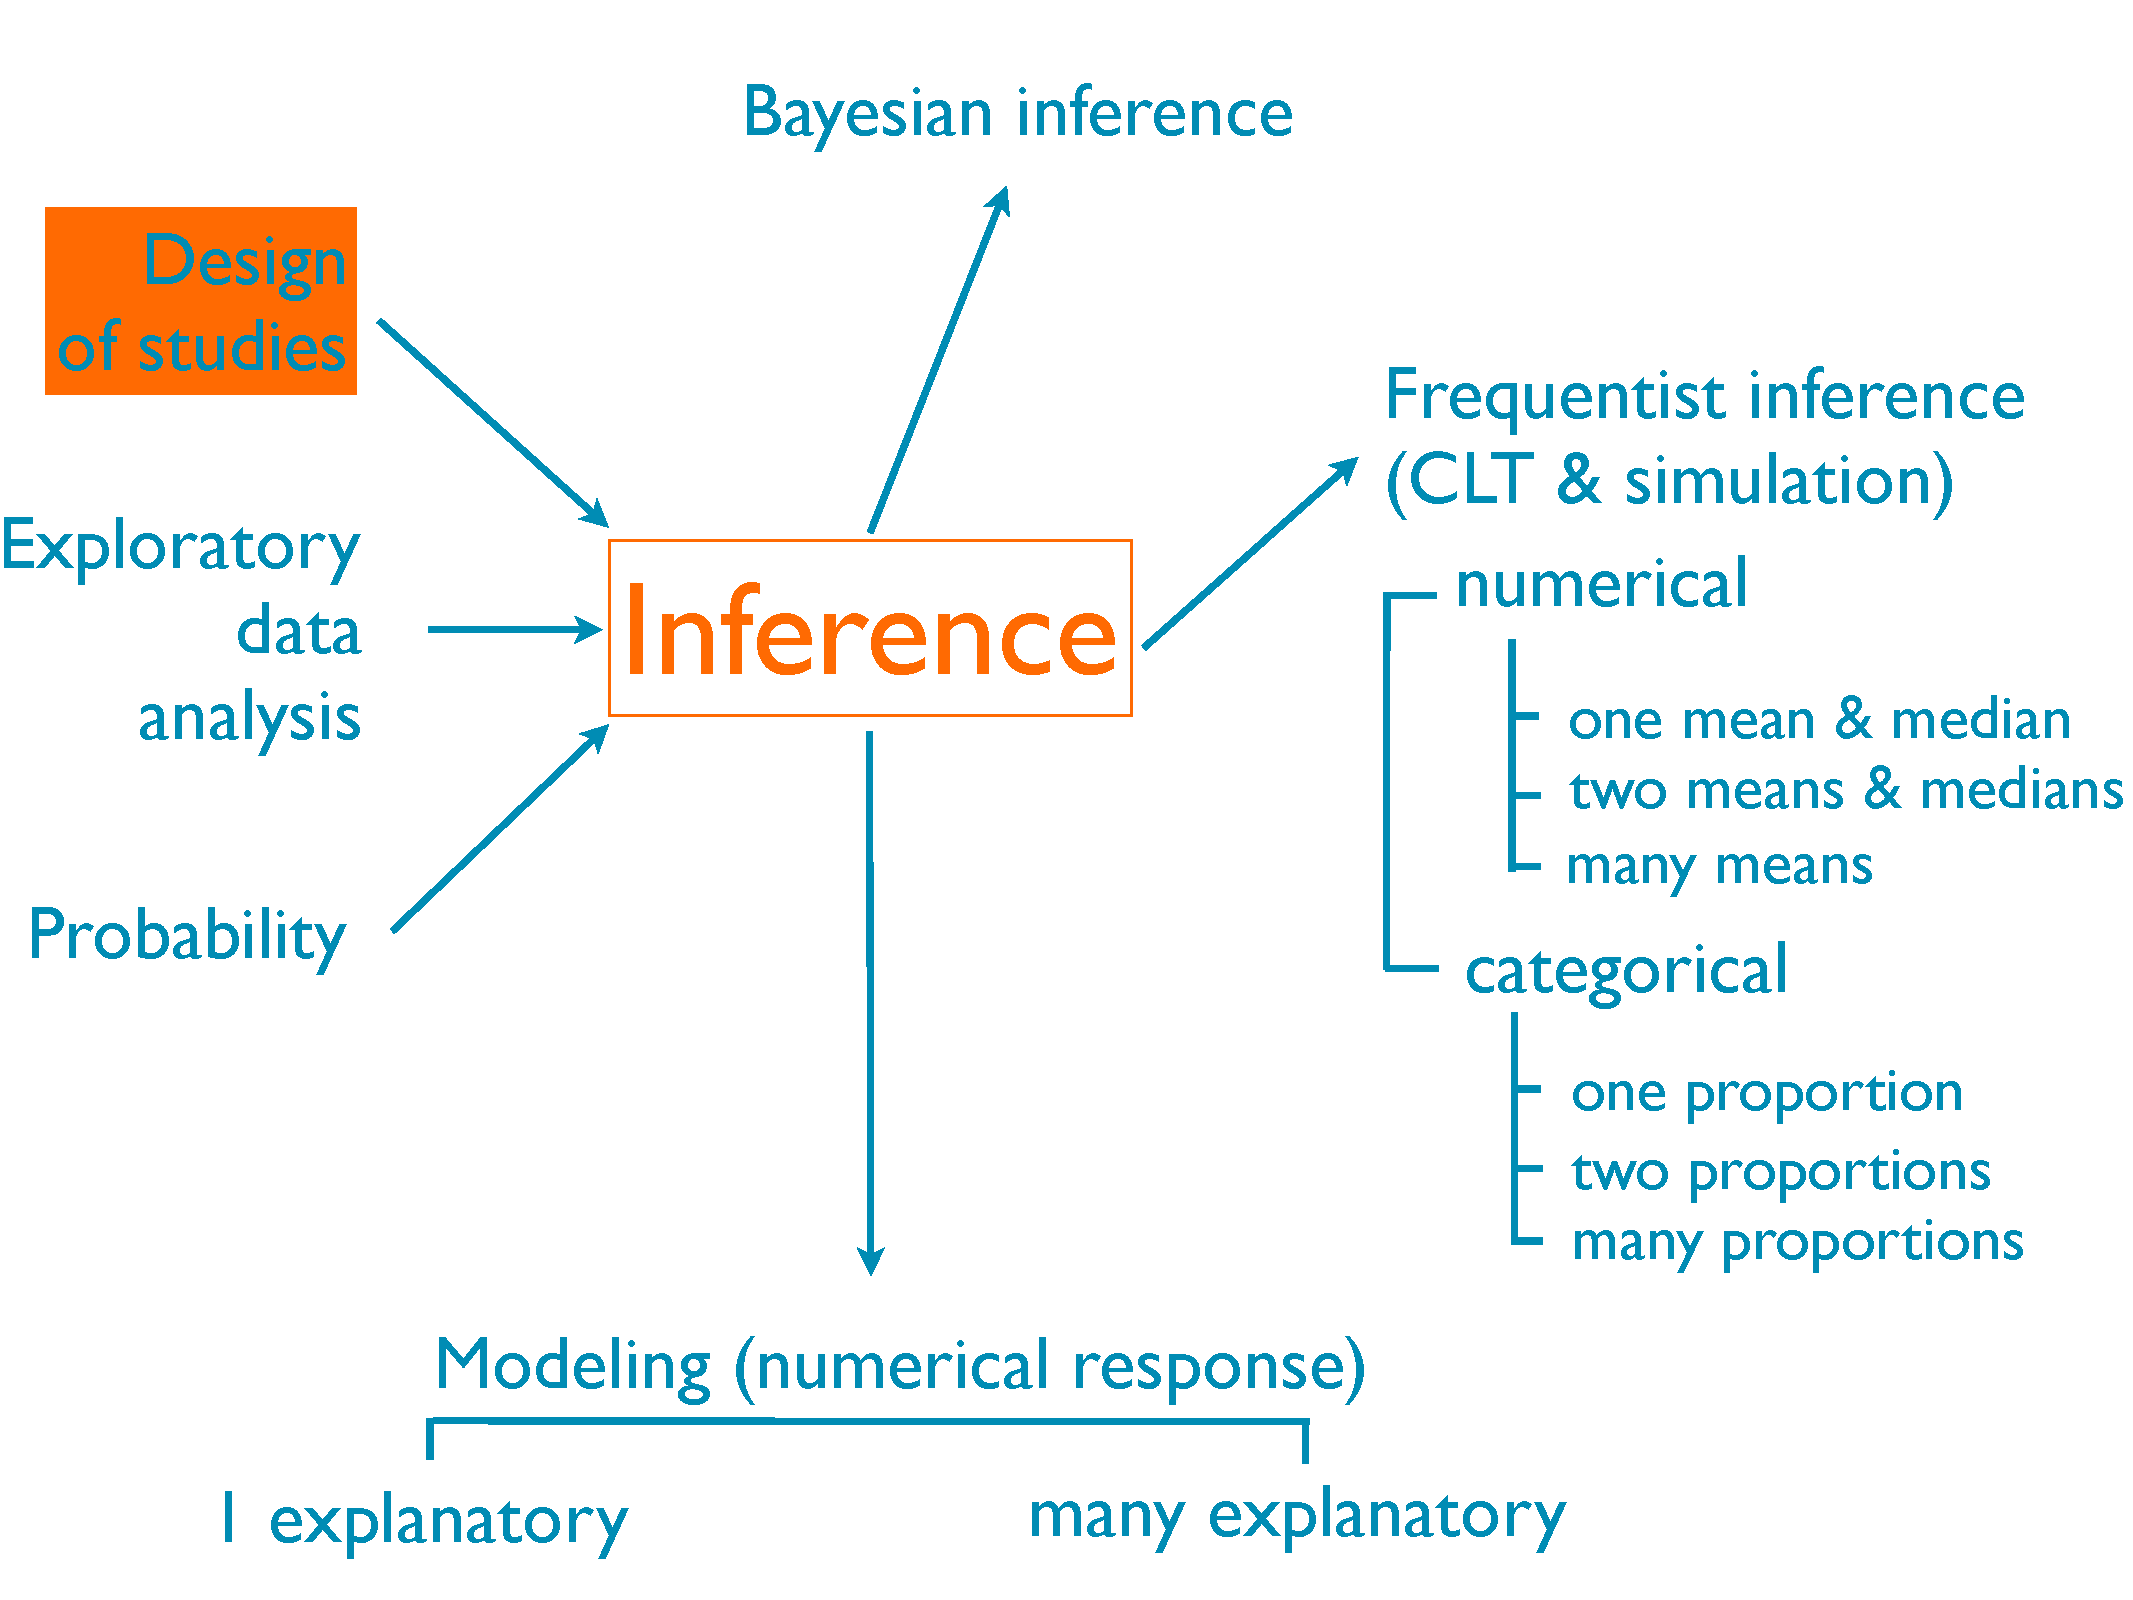
\includegraphics[width=\textwidth]{figures/map/design}
}

\vfill

{\footnotesize
\begin{enumerate}[(a)]
\item To prevent skewness in the results.
\item To reduce the amount of sampling variability.
\item To ensure that all potential cancer patients had an equal chance of being selected for the study.
\item \solnMult{To produce treatment groups with similar characteristics.}
\item To ensure that the sample is representative of all cancer patients.
\end{enumerate}
}

\end{frame}

%%%%%%%%%%%%%%%%%%%%%%%%%%%%%%%%%%%%

\begin{frame}

\twocol{0.7}{0.3}
{
{\scriptsize
\clicker{Which of the following is the most appropriate visualization for evaluating the relationship between a numerical and a categorical variable?
}}}
{
 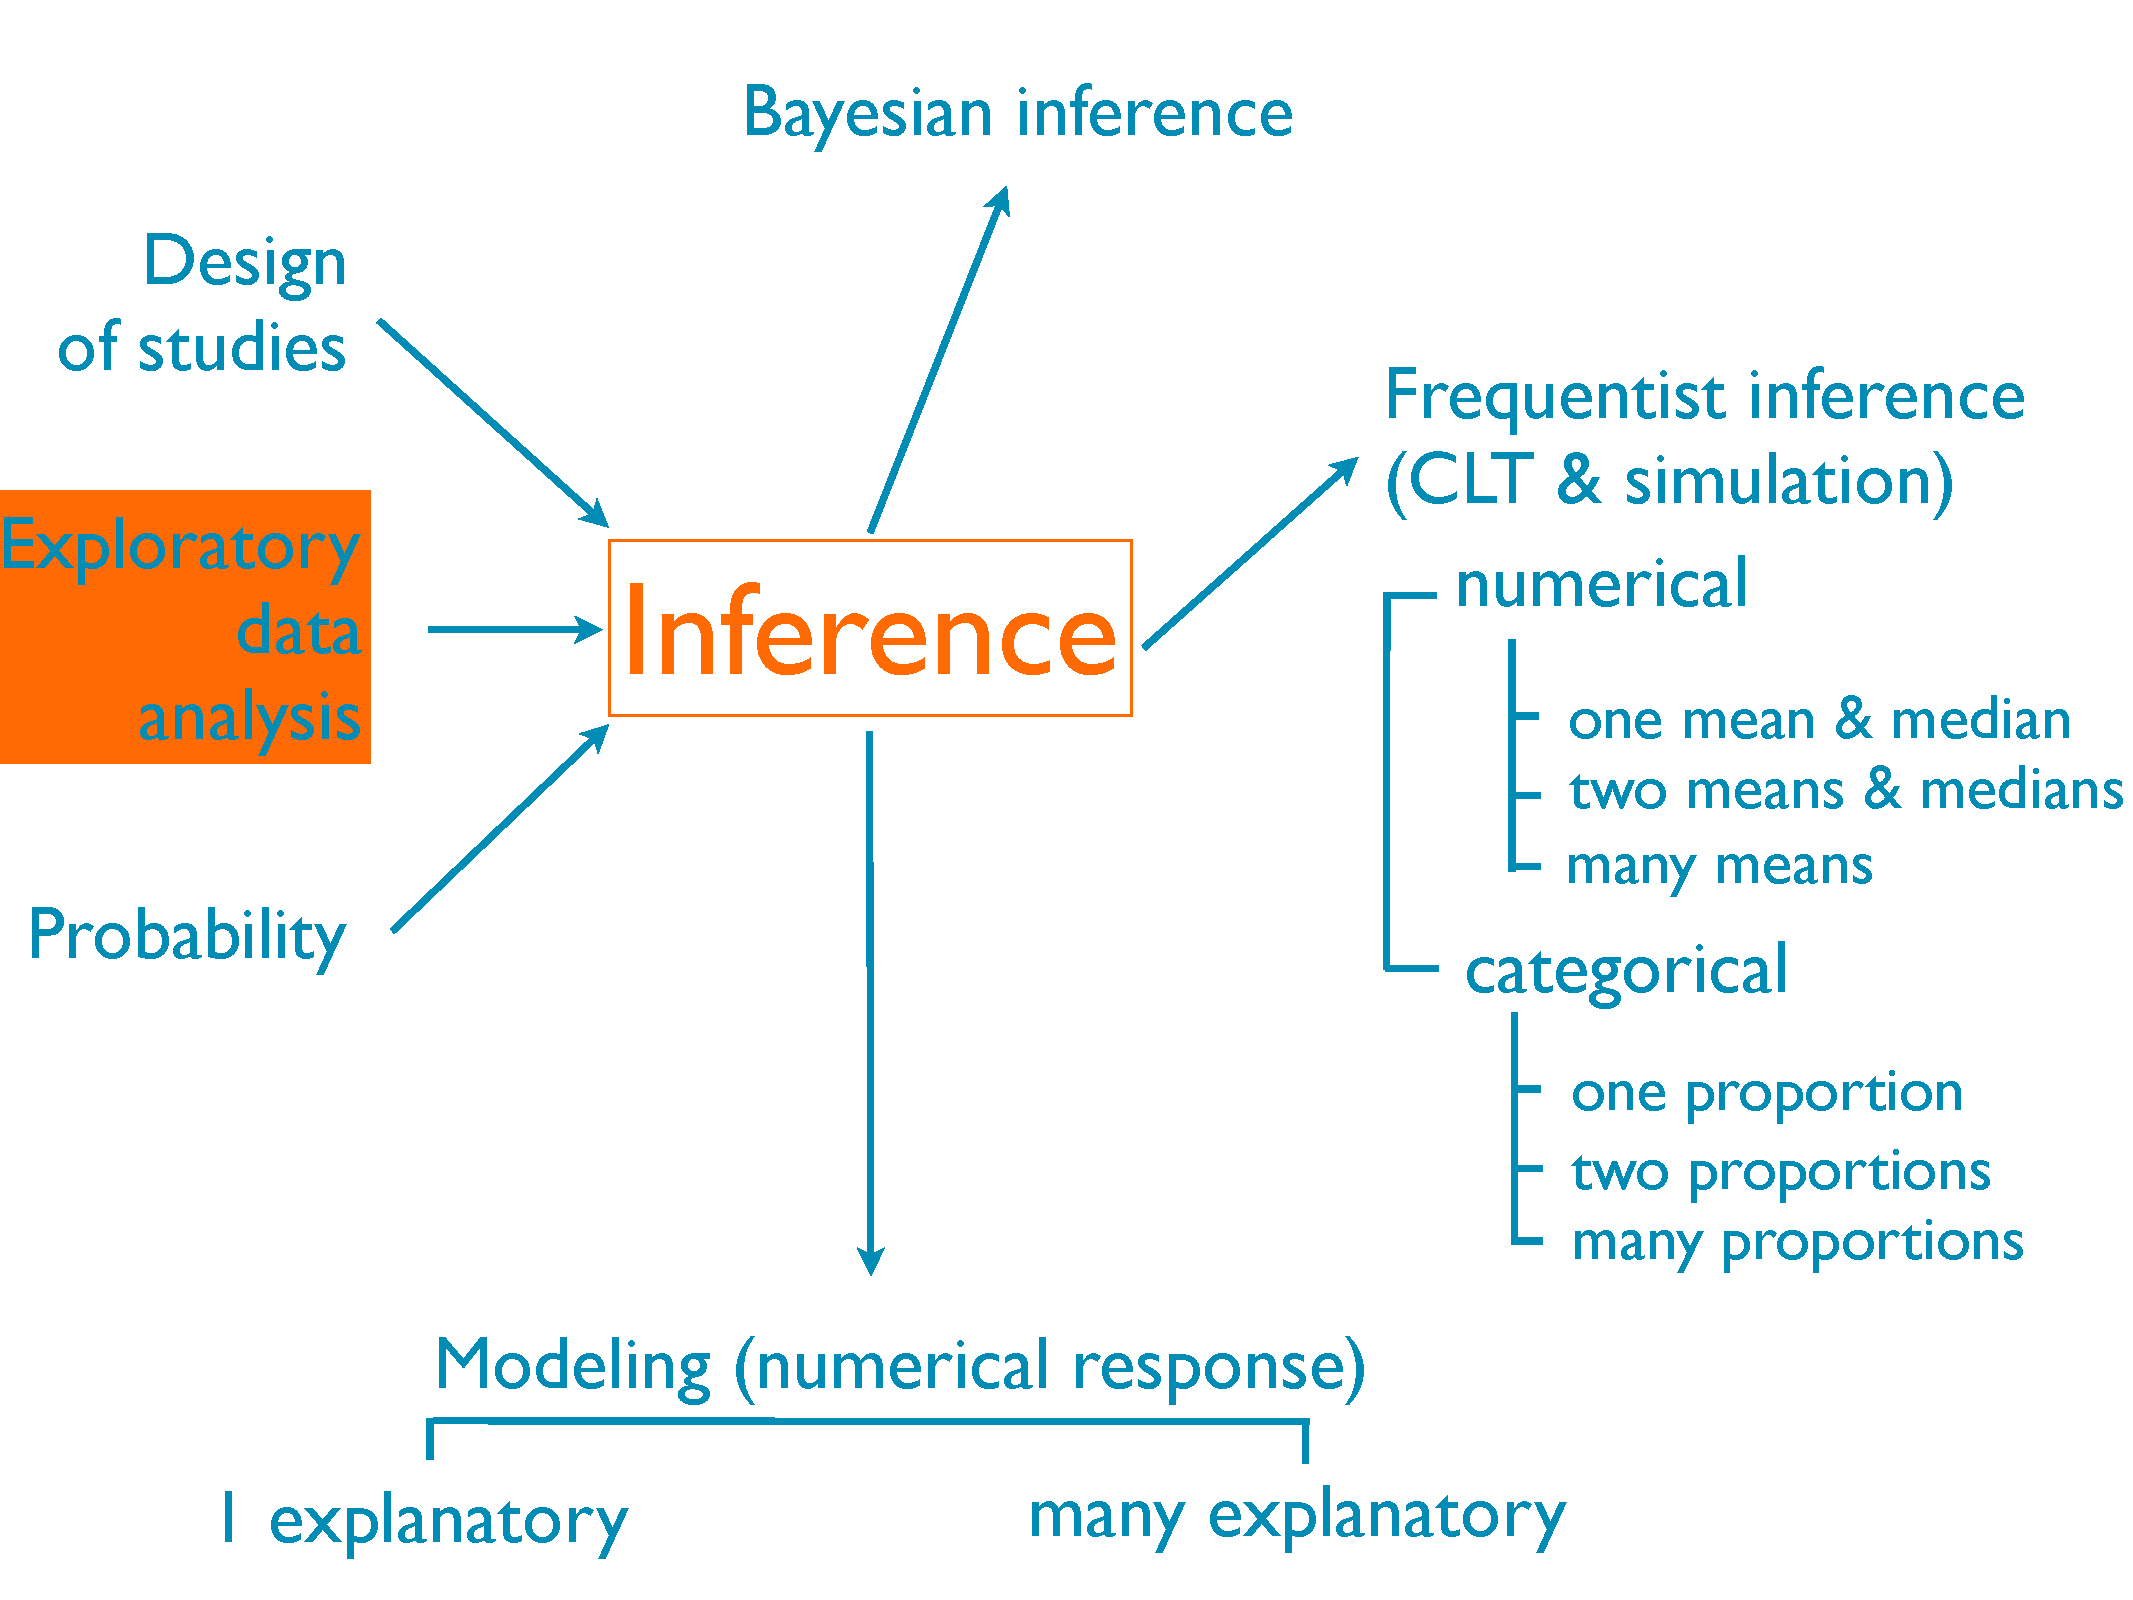
\includegraphics[width=\textwidth]{figures/map/eda}
}

\vfill

{\footnotesize
\begin{enumerate}[(a)]
\item a mosaic plot
\item a segmented frequency bar plot
\item a frequency histogram
\item a relative frequency histogram
\item \solnMult{side-by-side box plots}
\end{enumerate}
}

\end{frame}

%%%%%%%%%%%%%%%%%%%%%%%%%%%%%%%%%%%%

\begin{frame}

\twocol{0.7}{0.3}
{
{\scriptsize
\clicker{Which of the following is \underline{false}?
}}}
{
 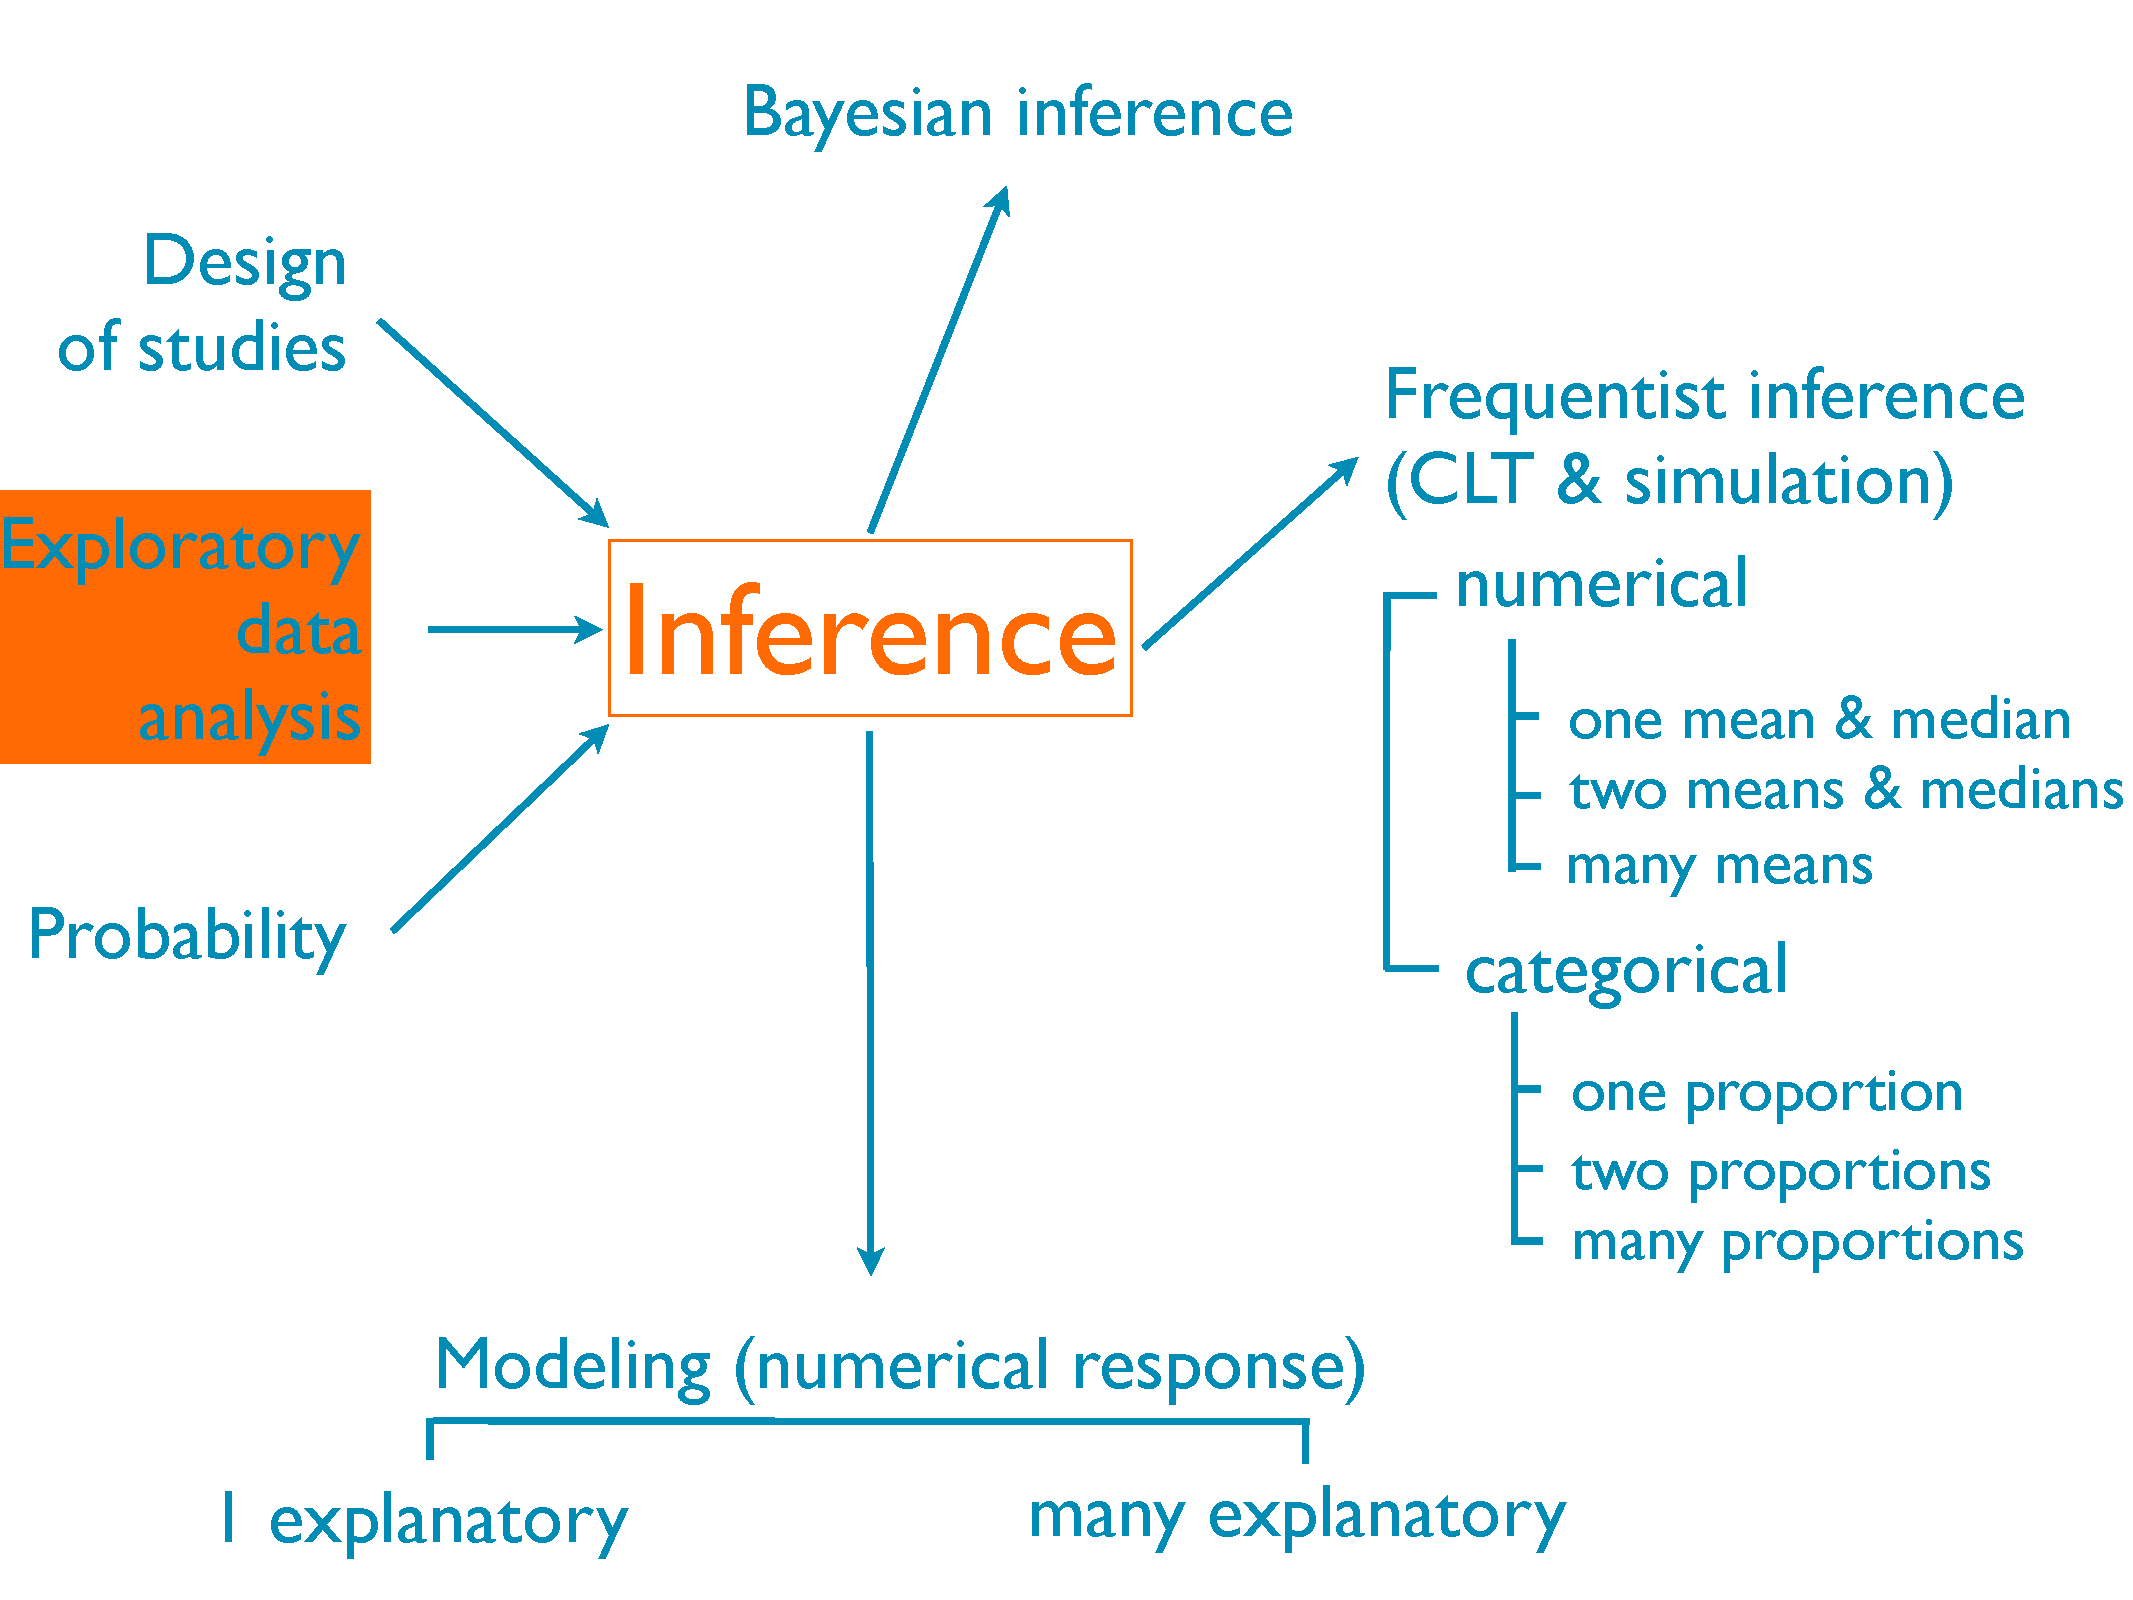
\includegraphics[width=\textwidth]{figures/map/eda}
}

\vfill

{\footnotesize
\begin{enumerate}[(a)]
\item \solnMult{Box plots are useful for highlighting outliers, but we cannot determine skew based on a box plot.}
\item Median and IQR are more robust statistics than mean and SD, respectively, since they are not affected by outliers or extreme skewness.
\item When the response variable is extremely right skewed, it may be useful to apply a log transformation to obtain a more symmetric distribution, and model the logged data.
\item Segmented frequency bar plots are ``good enough" for evaluating the relationship between two categorical variables if the sample sizes are the same for various levels of the explanatory variable.
\end{enumerate}
}

\end{frame}

%%%%%%%%%%%%%%%%%%%%%%%%%%%%%%%%%%%%

\begin{frame}

\twocol{0.7}{0.3}
{
{\scriptsize
\clicker{Which of the following is \underline{false}?
}}}
{
 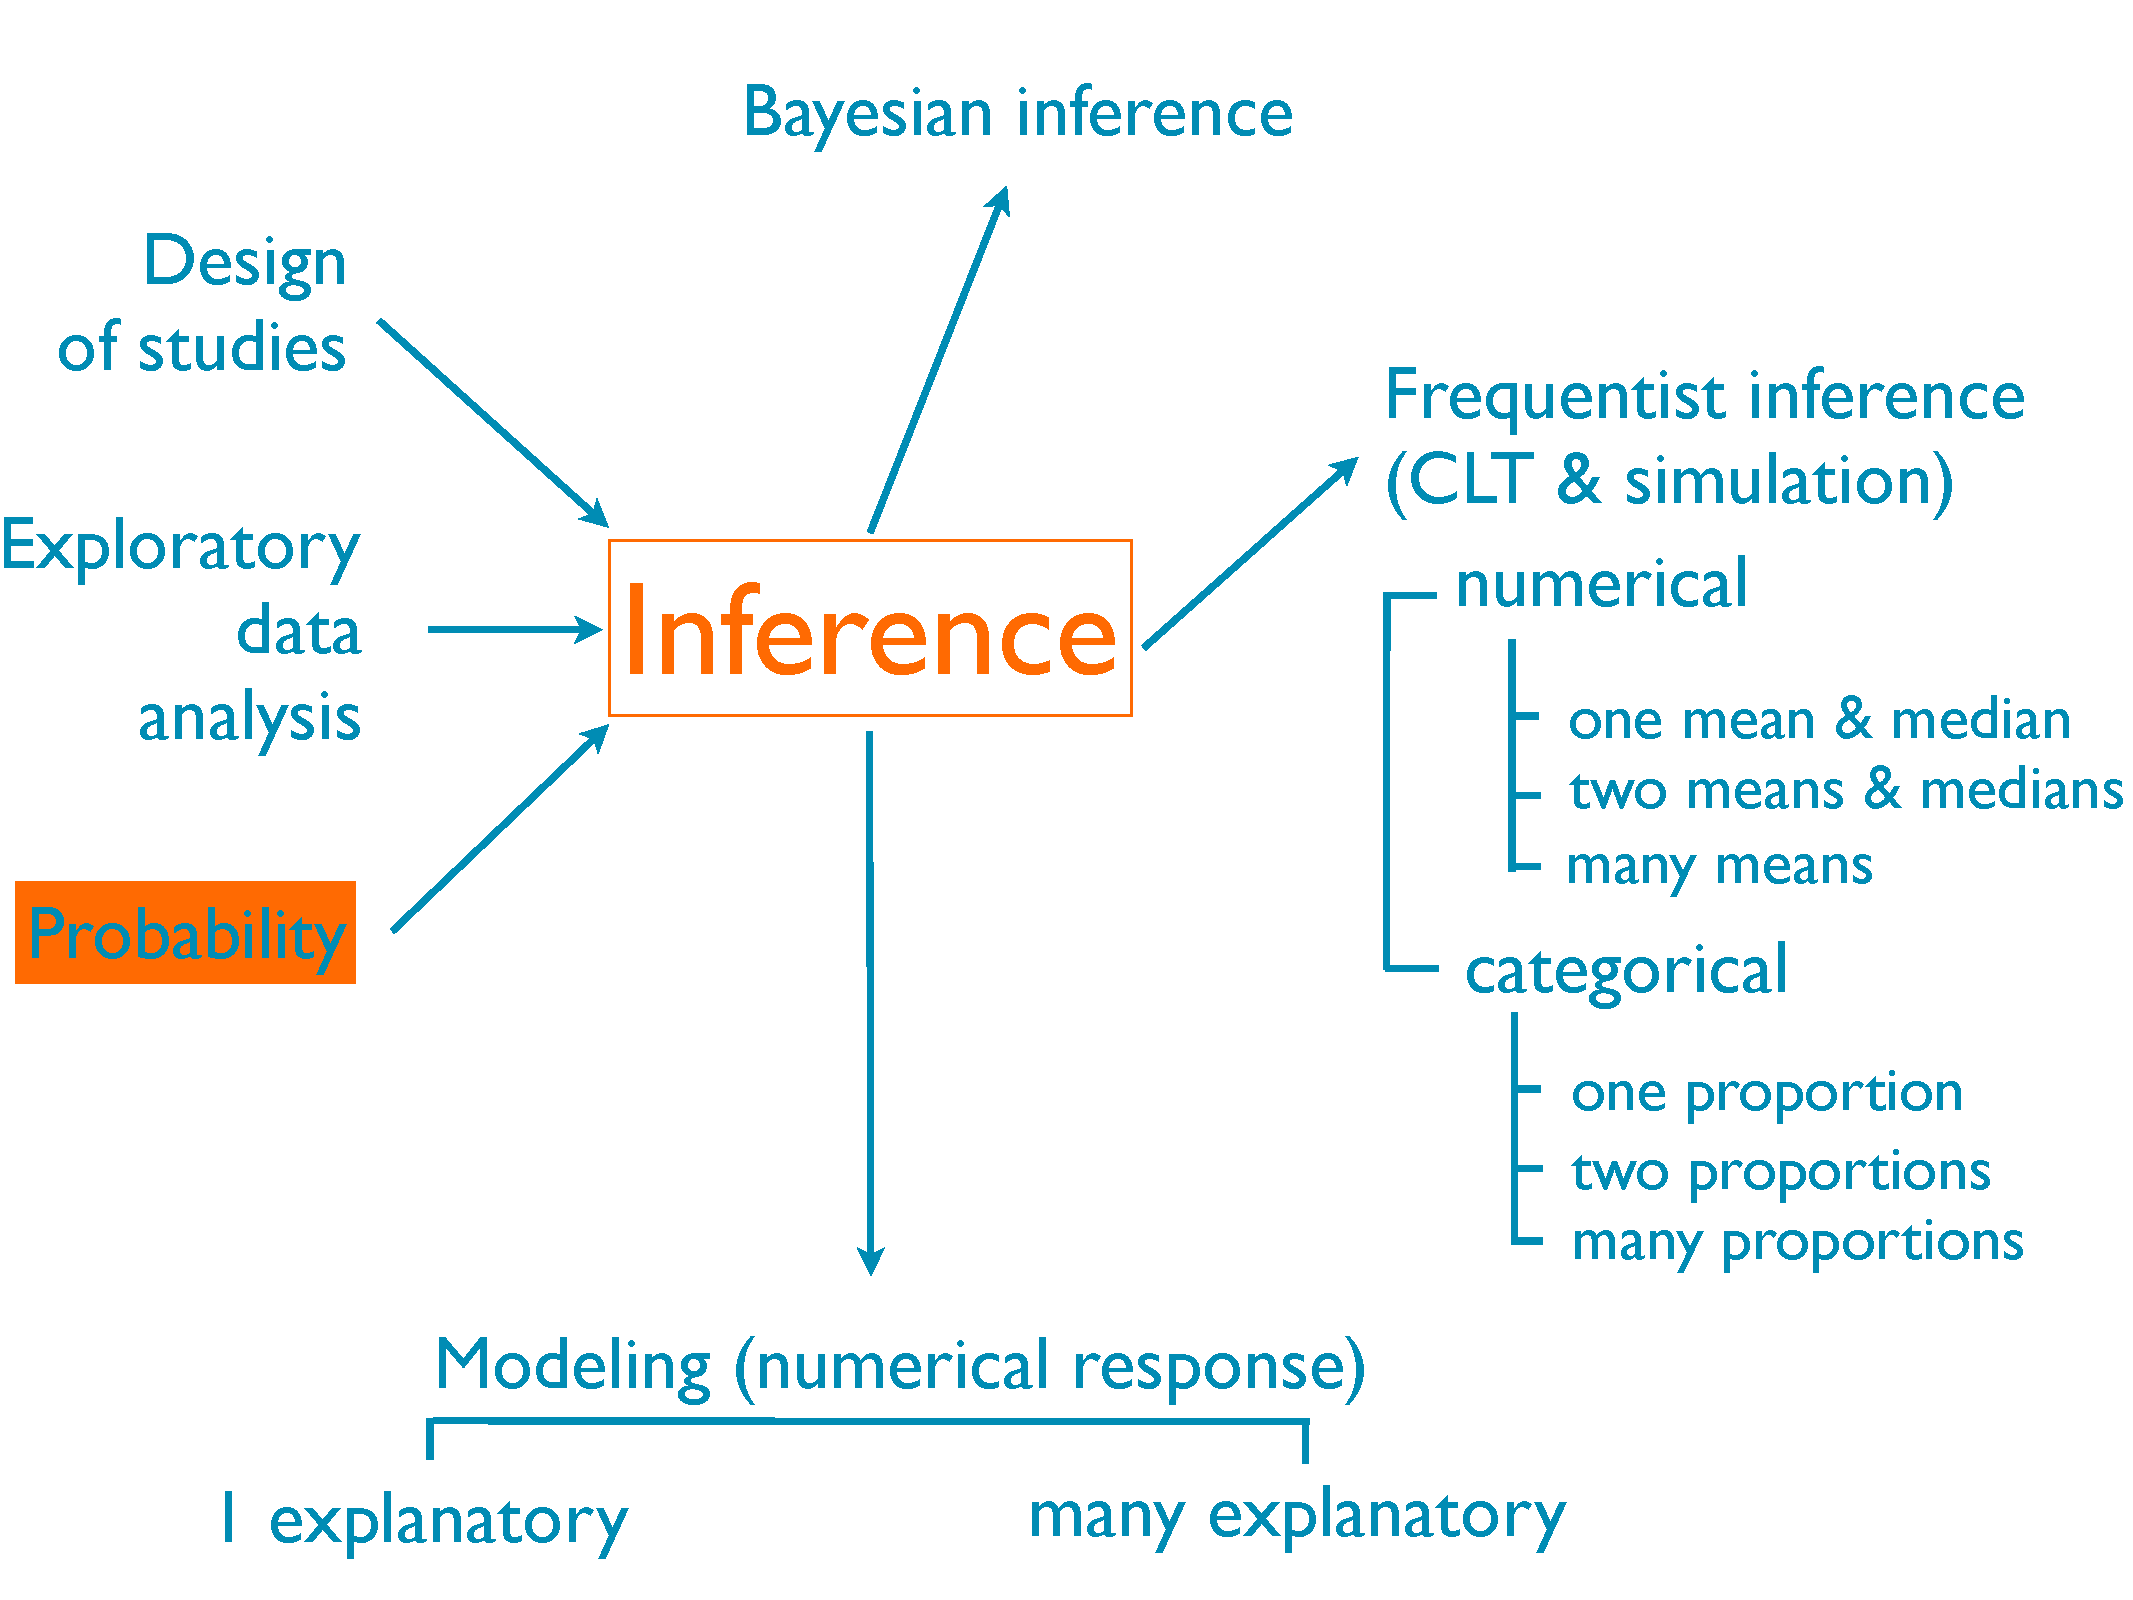
\includegraphics[width=\textwidth]{figures/map/probability}
}

\vfill

{\footnotesize
\begin{enumerate}[(a)]
\item If A and B are independent, then having information on A does not tell us anything about B.
\item If A and B are disjoint, then knowing that A occurs tells us that B cannot occur.
\item Disjoint (mutually exclusive) events are always dependent since if one event occurs we know the other one cannot.
\item \solnMult{If A and B are independent, then P(A and B) = P(A) + P(B).}
\item If A and B are not disjoint, then P(A or B) = P(A) + P(B) - P(A and B).
\end{enumerate}
}

\end{frame}

%%%%%%%%%%%%%%%%%%%%%%%%%%%%%%%%%%%%

\begin{frame}

\twocol{0.7}{0.3}
{
{\scriptsize
\disc{About 30\% of human twins are identical and the rest are fraternal. Identical twins are necessarily the same sex -- half are males and the other half are females. One-quarter of fraternal twins are both male, one-quarter both female, and one-half are mixes: one male, one female. You have just become a parent of twins and are told they are both girls. Given this information, what is the posterior probability that they are identical?}}}
{
 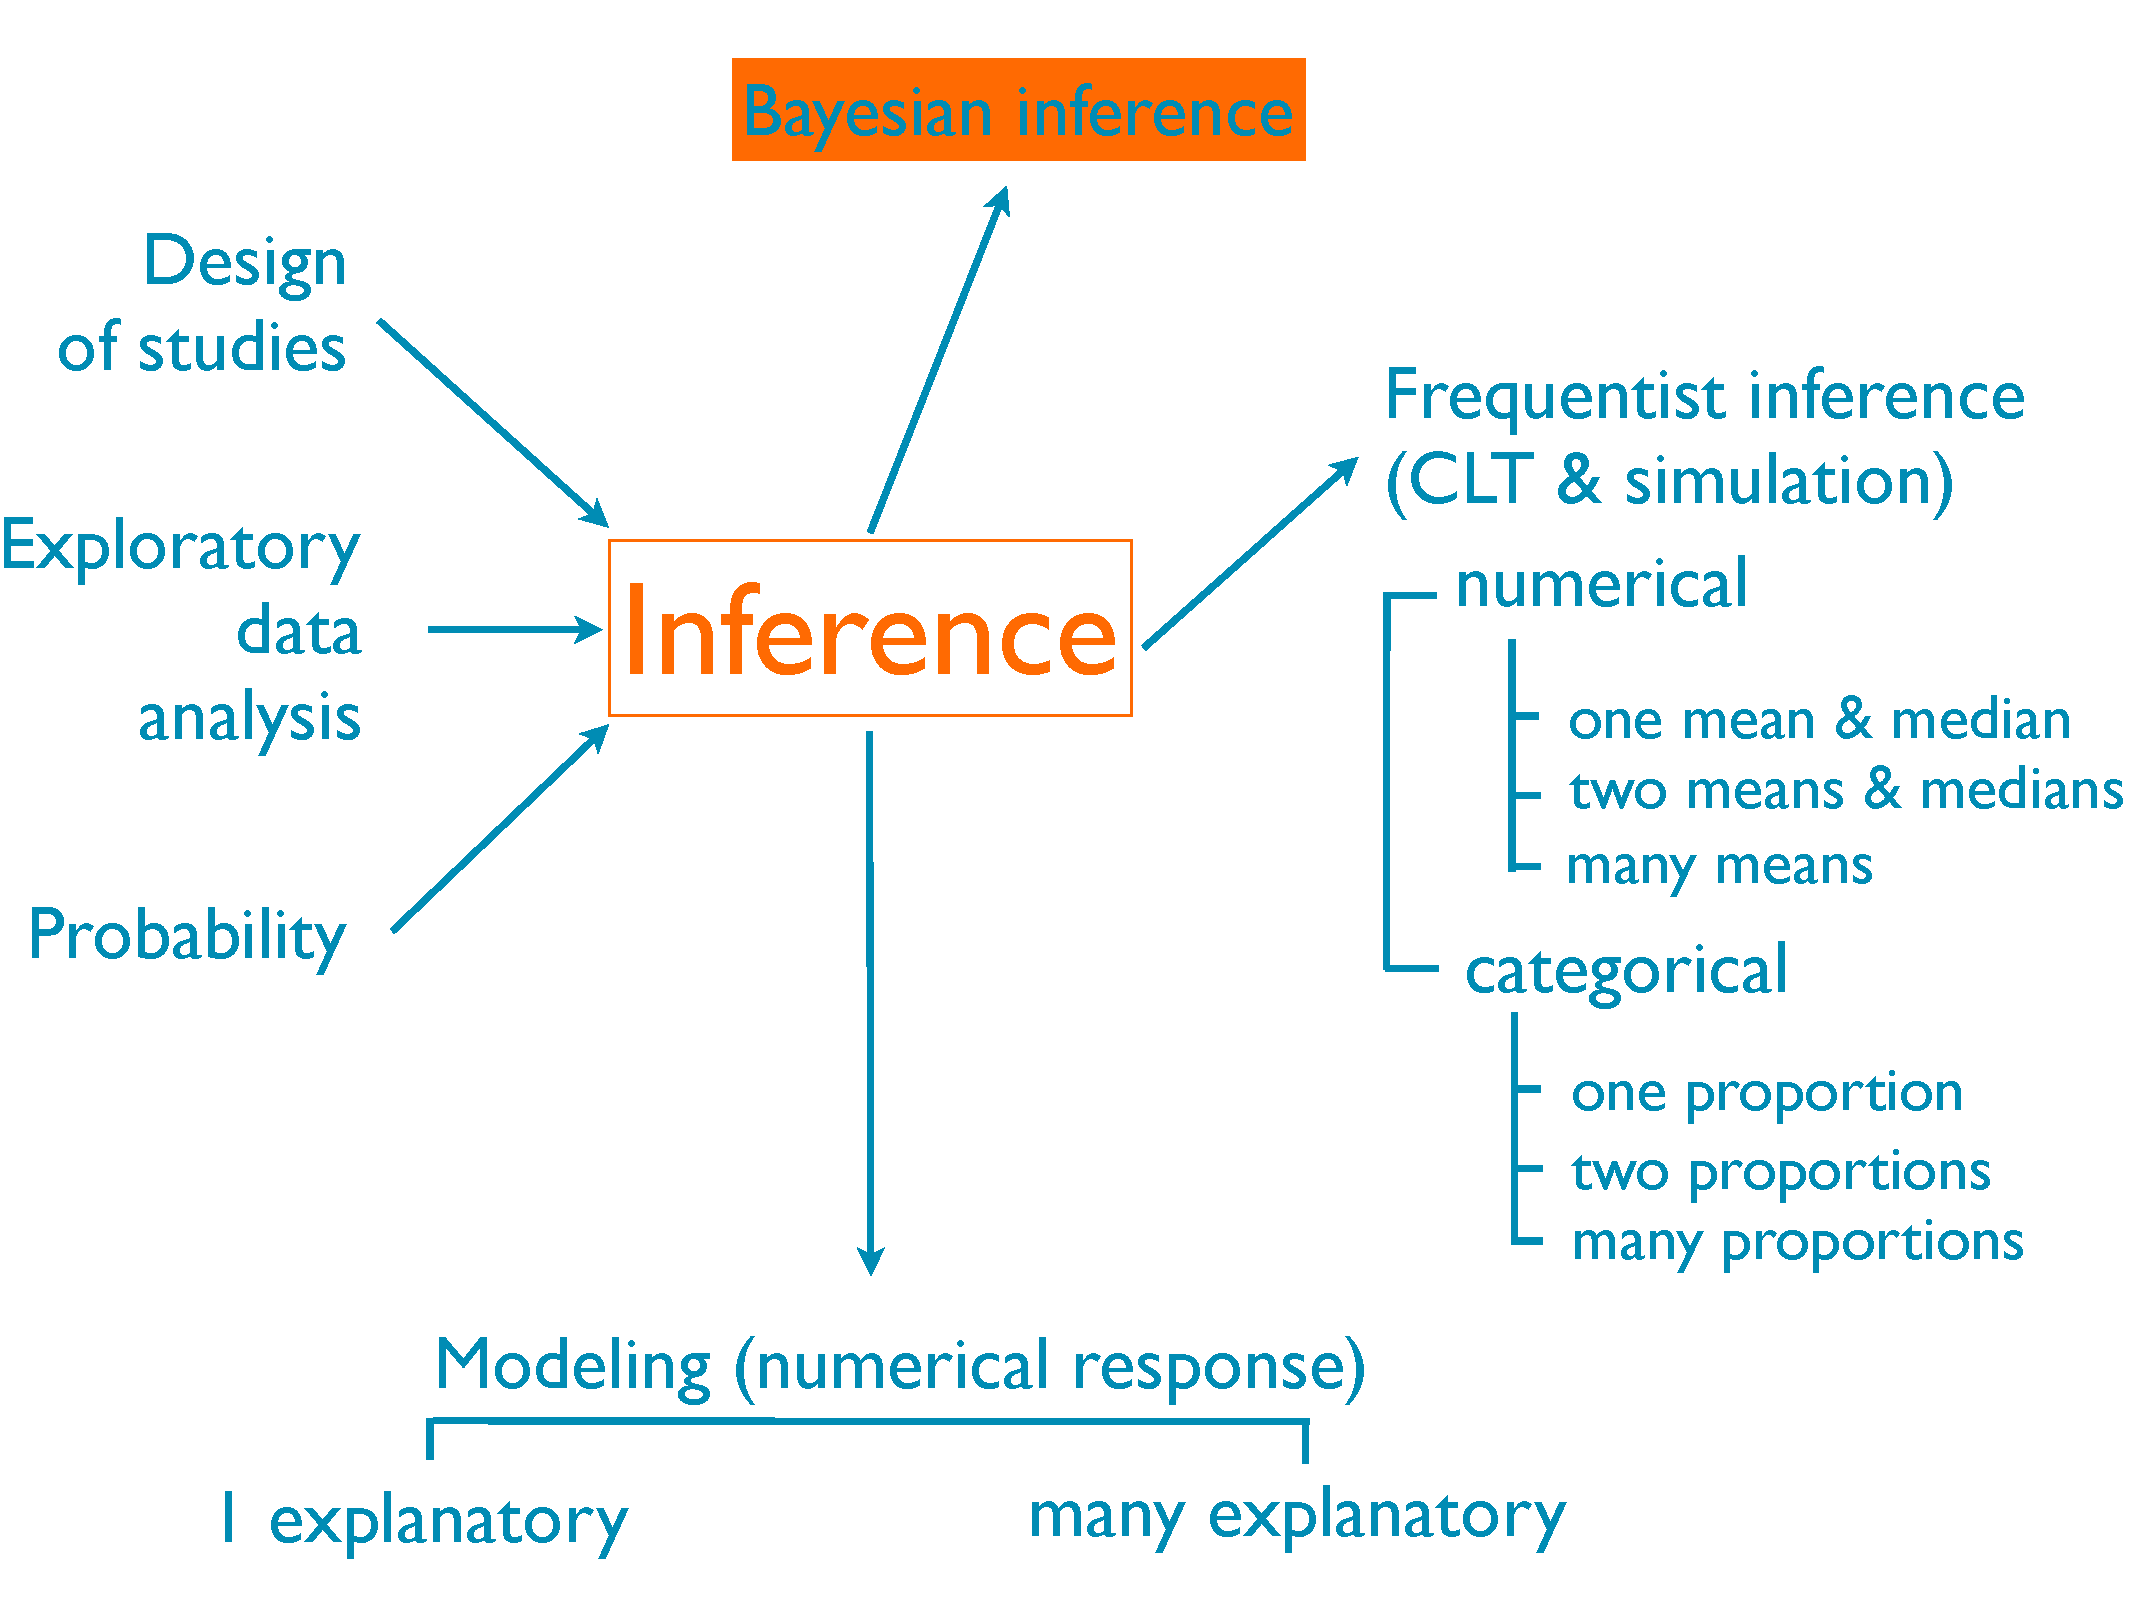
\includegraphics[width=\textwidth]{figures/map/bayes}
}

\pause
\vspace{-1cm}

\twocol{0.6}{0.4}
{
\begin{center}
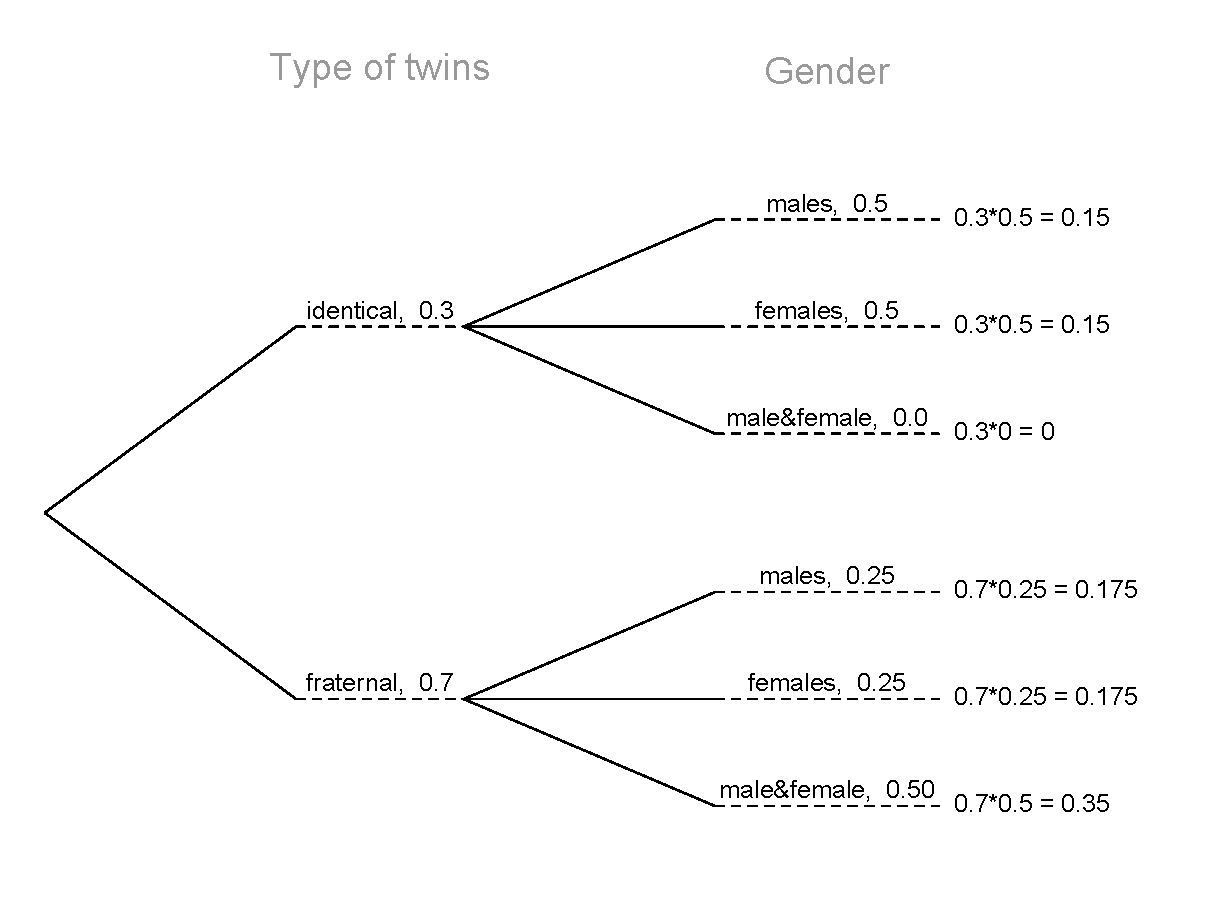
\includegraphics[width =1.1\textwidth]{figures/twins_tree}
\end{center}
}
{
\pause
{\small
\begin{eqnarray*}
P(iden~|~f) &=& \frac{P(iden~\&~f)}{P(f)} \\
\pause
&=& \frac{0.15}{0.15+0.175} \\
\pause
&=& 0.46
\end{eqnarray*}
}
}

\end{frame}

%%%%%%%%%%%%%%%%%%%%%%%%%%%%%%%%%%%%

\begin{frame}

\twocol{0.7}{0.3}
{
{\scriptsize
\clicker{Which of the following is \underline{false}?}}}
{
 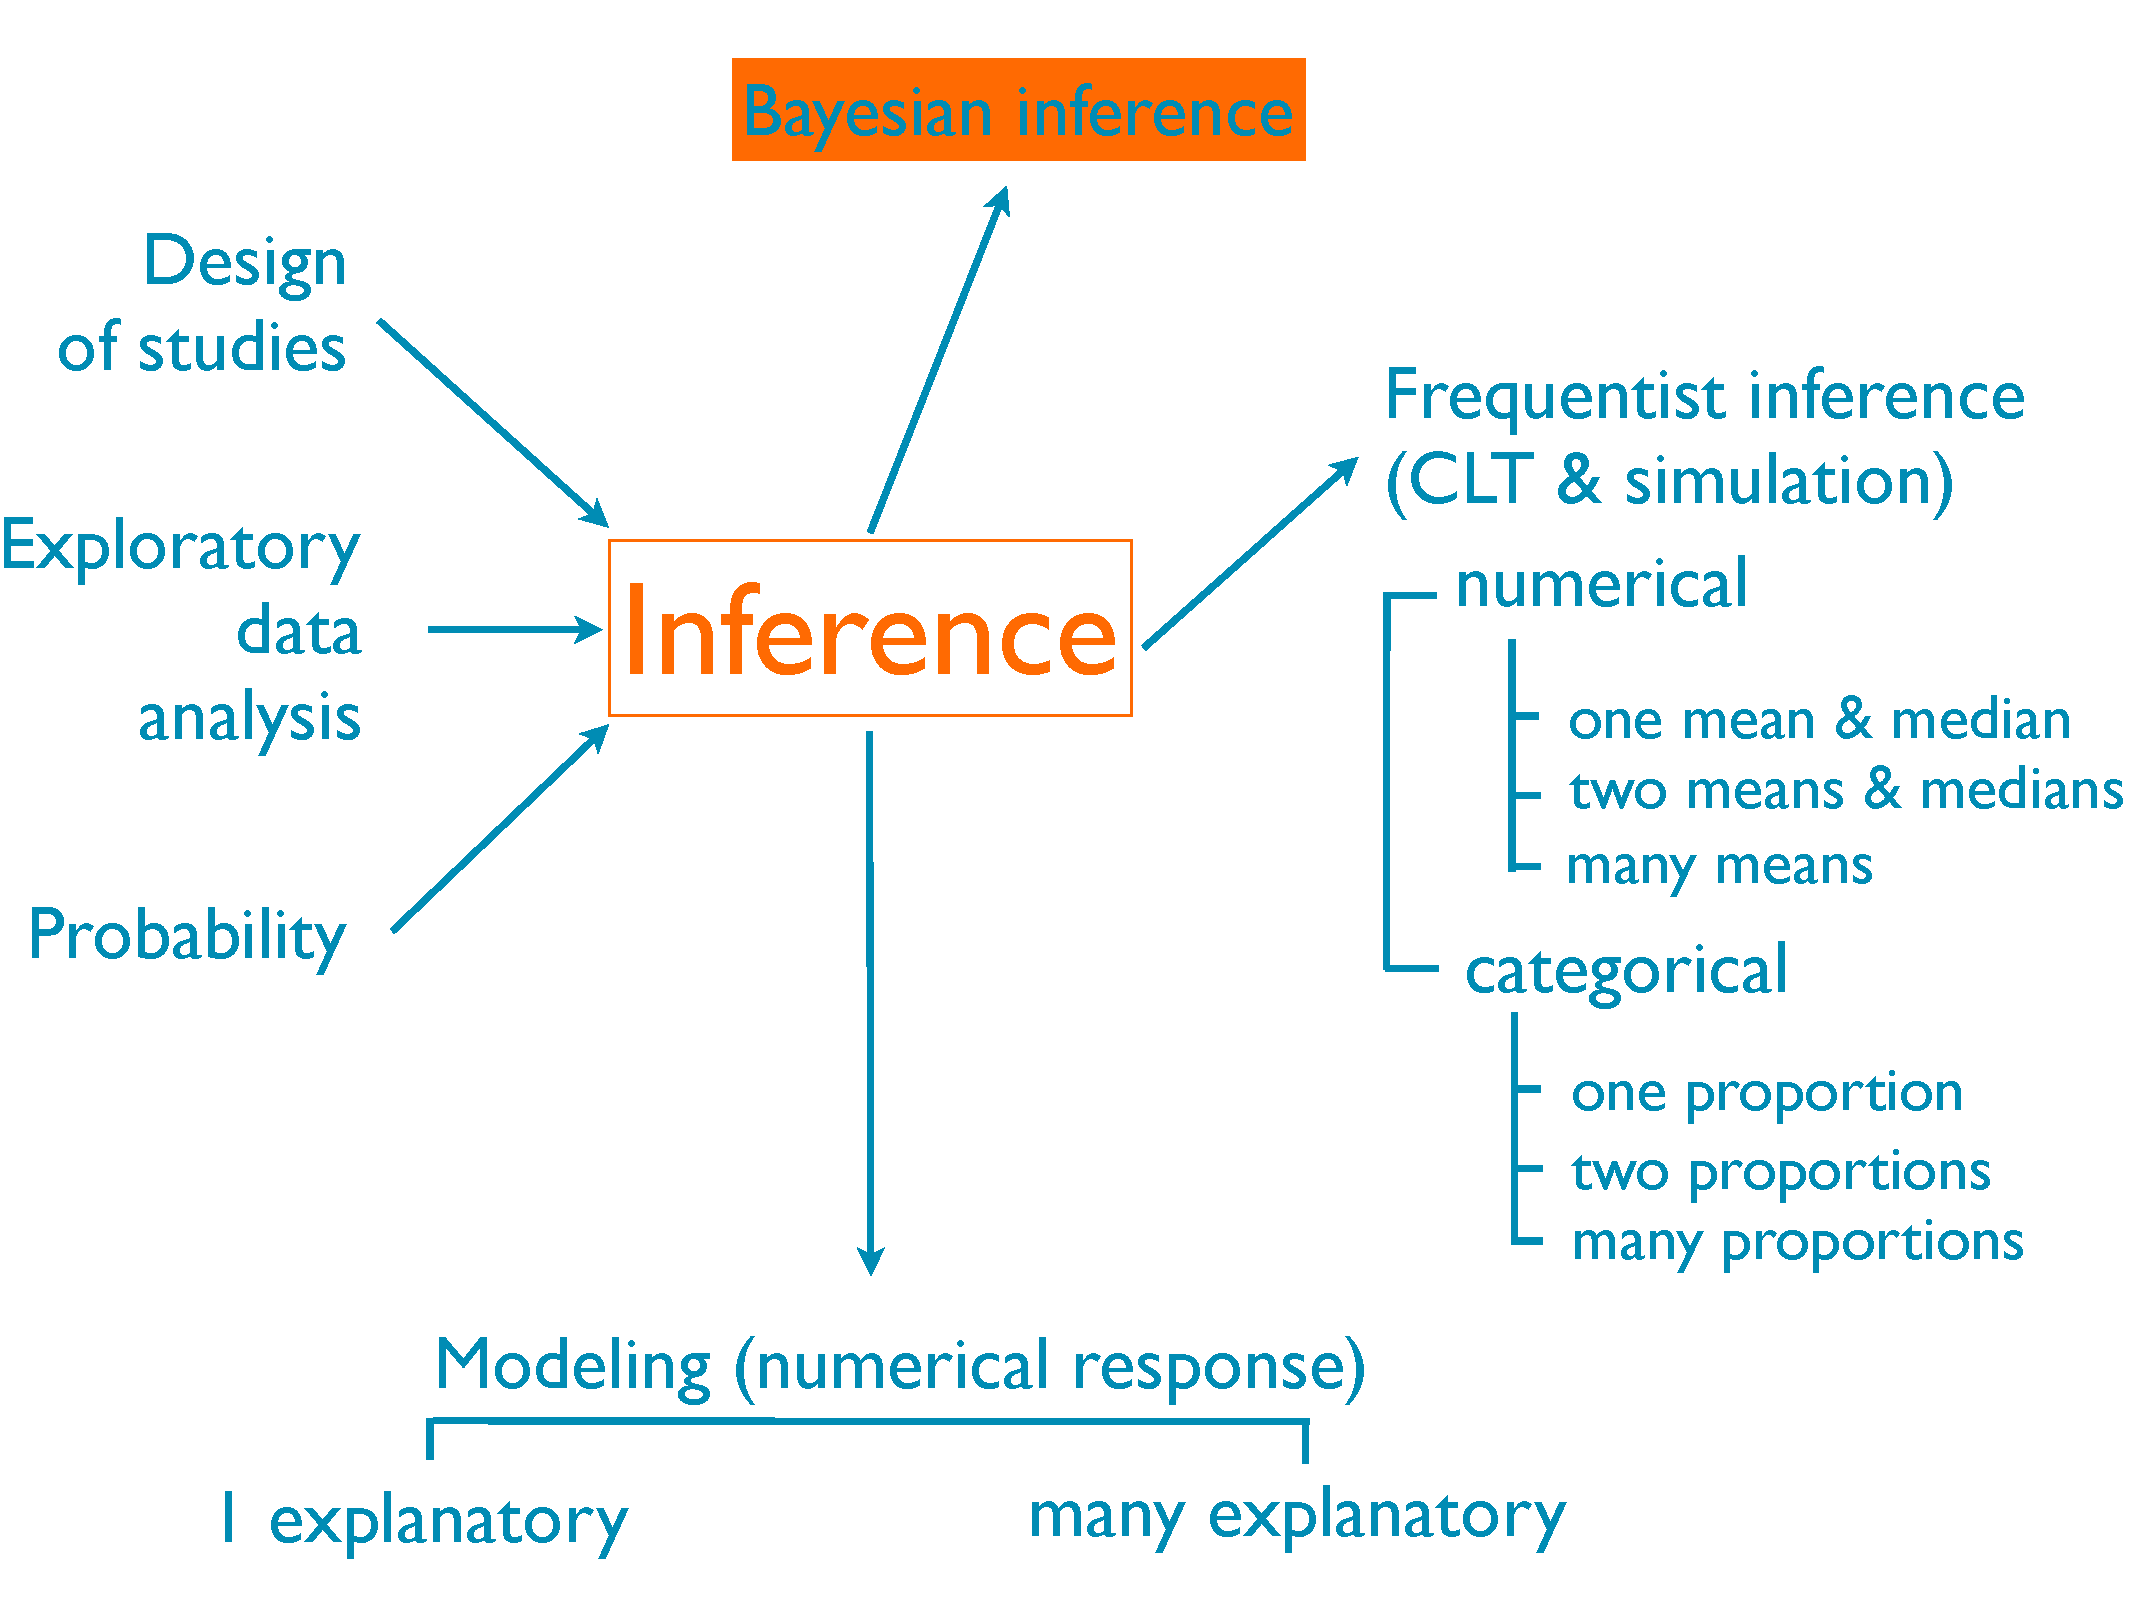
\includegraphics[width=\textwidth]{figures/map/bayes}
}

\begin{enumerate}[(a)]
\item Suppose you're evaluating 4 claims. If prior to data collection you don't have a preference for one claim over another, you should assign 0.25 as the prior probability to each claim.
\item \solnMult{Posterior probability and the p-value are the equivalent.}
\item One advantage of Bayesian inference is that data can be integrated to the inferential scheme as they are collected.
\item Suppose a patient tests positive for a disease that 2\% of the population are known to have. A doctor wants to confirm the test result by retesting the patient. In the second test the prior probability for ``having the disease" should be more than 2\%.
\end{enumerate}

\pause
\soln{\red{Posterior = P(hypothesis $|$ data), p-value $\approx$ P(data $|$ hypothesis)}}

\end{frame}

%%%%%%%%%%%%%%%%%%%%%%%%%%%%%%%%%%%%

\begin{frame}

\vspace{-0.25cm}

\activity{}{Test the hypothesis $H_0: \mu = 10$ vs. $H_A: \mu > 10$ for the following 6 samples. Assume $\sigma = 2$.}

\vspace{-0.25cm}

\begin{center}
\renewcommand\arraystretch{1}
\begin{tabular}{l | c | c | c | c}
\hline
$\bar{x}$		& $10.05$ 	& $10.1$ 		& $10.2$  		 \\
\hline
\hline
\red{$n = 30$} 	& {\tiny 8:30am section}			& {\tiny 10:05am section}			& {\tiny 11:45am section} \\
\hline
$p-value$		& \soln{\only<2->{$0.45$}}	& \soln{\only<4->{$0.39$}} 		& \soln{\only<6->{$29$}} \\
\hline
\hline
\red{$n = 5000$} & {\tiny 1:25pm section}			& {\tiny 3:05pm section}			& {\tiny 4:40pm section} \\
\hline
$p-value$		&  \soln{\only<3->{$0.04$}}	& \soln{\only<5->{$0.0002$}}	& \soln{\only<7->{$\approx0$}}	 \\
\hline
\end{tabular}
\end{center}

\pause

\end{frame}

%%%%%%%%%%%%%%%%%%%%%%%%%%%%%%%%%%%%

\begin{frame}

\twocol{0.7}{0.3}
{
{\scriptsize
\clicker{Which of the following is the best method for evaluating the if the distribution of a categorical variable follows a hypothesized distribution?}}}
{
 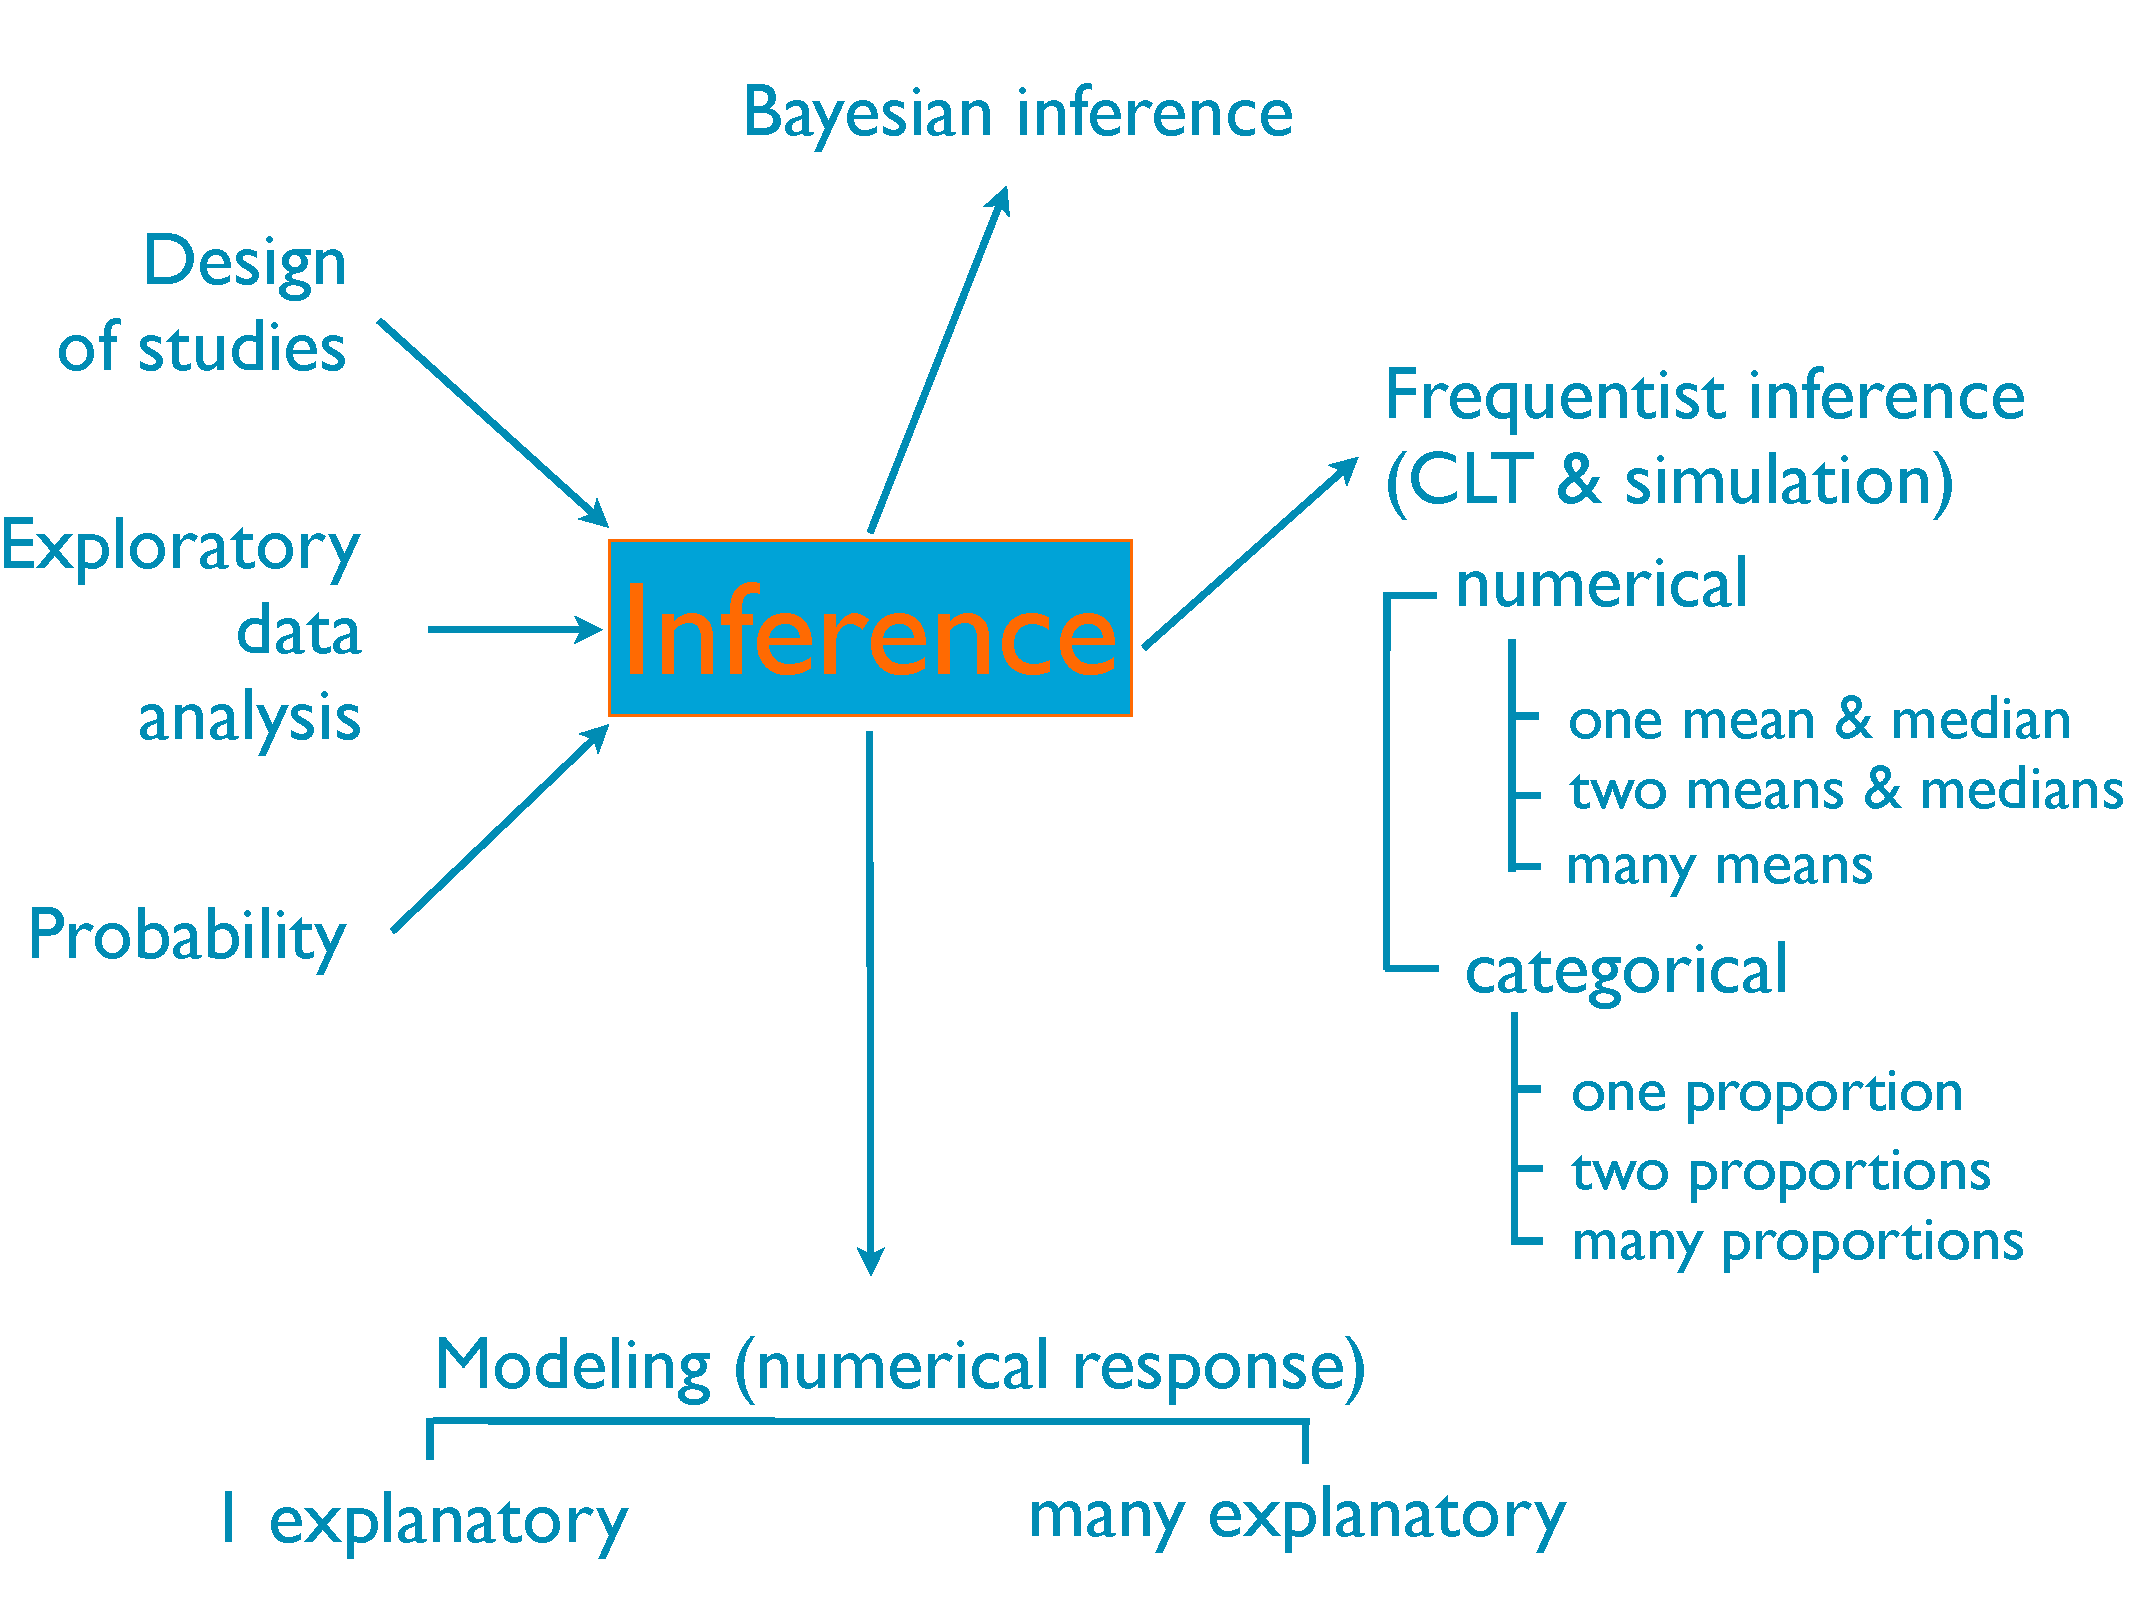
\includegraphics[width=\textwidth]{figures/map/inference}
}

\begin{enumerate}[(a)]
\item chi-square test of independence
\item \solnMult{chi-square test of goodness of fit}
\item anova
\item linear regression
\item t-test
\end{enumerate}

\end{frame}

%%%%%%%%%%%%%%%%%%%%%%%%%%%%%%%%%%%%

\begin{frame}

\twocol{0.7}{0.3}
{
{\scriptsize
\clicker{Which of the following is the best method for evaluating the relationship between a numerical and a categorical variable with many levels?}}}
{
 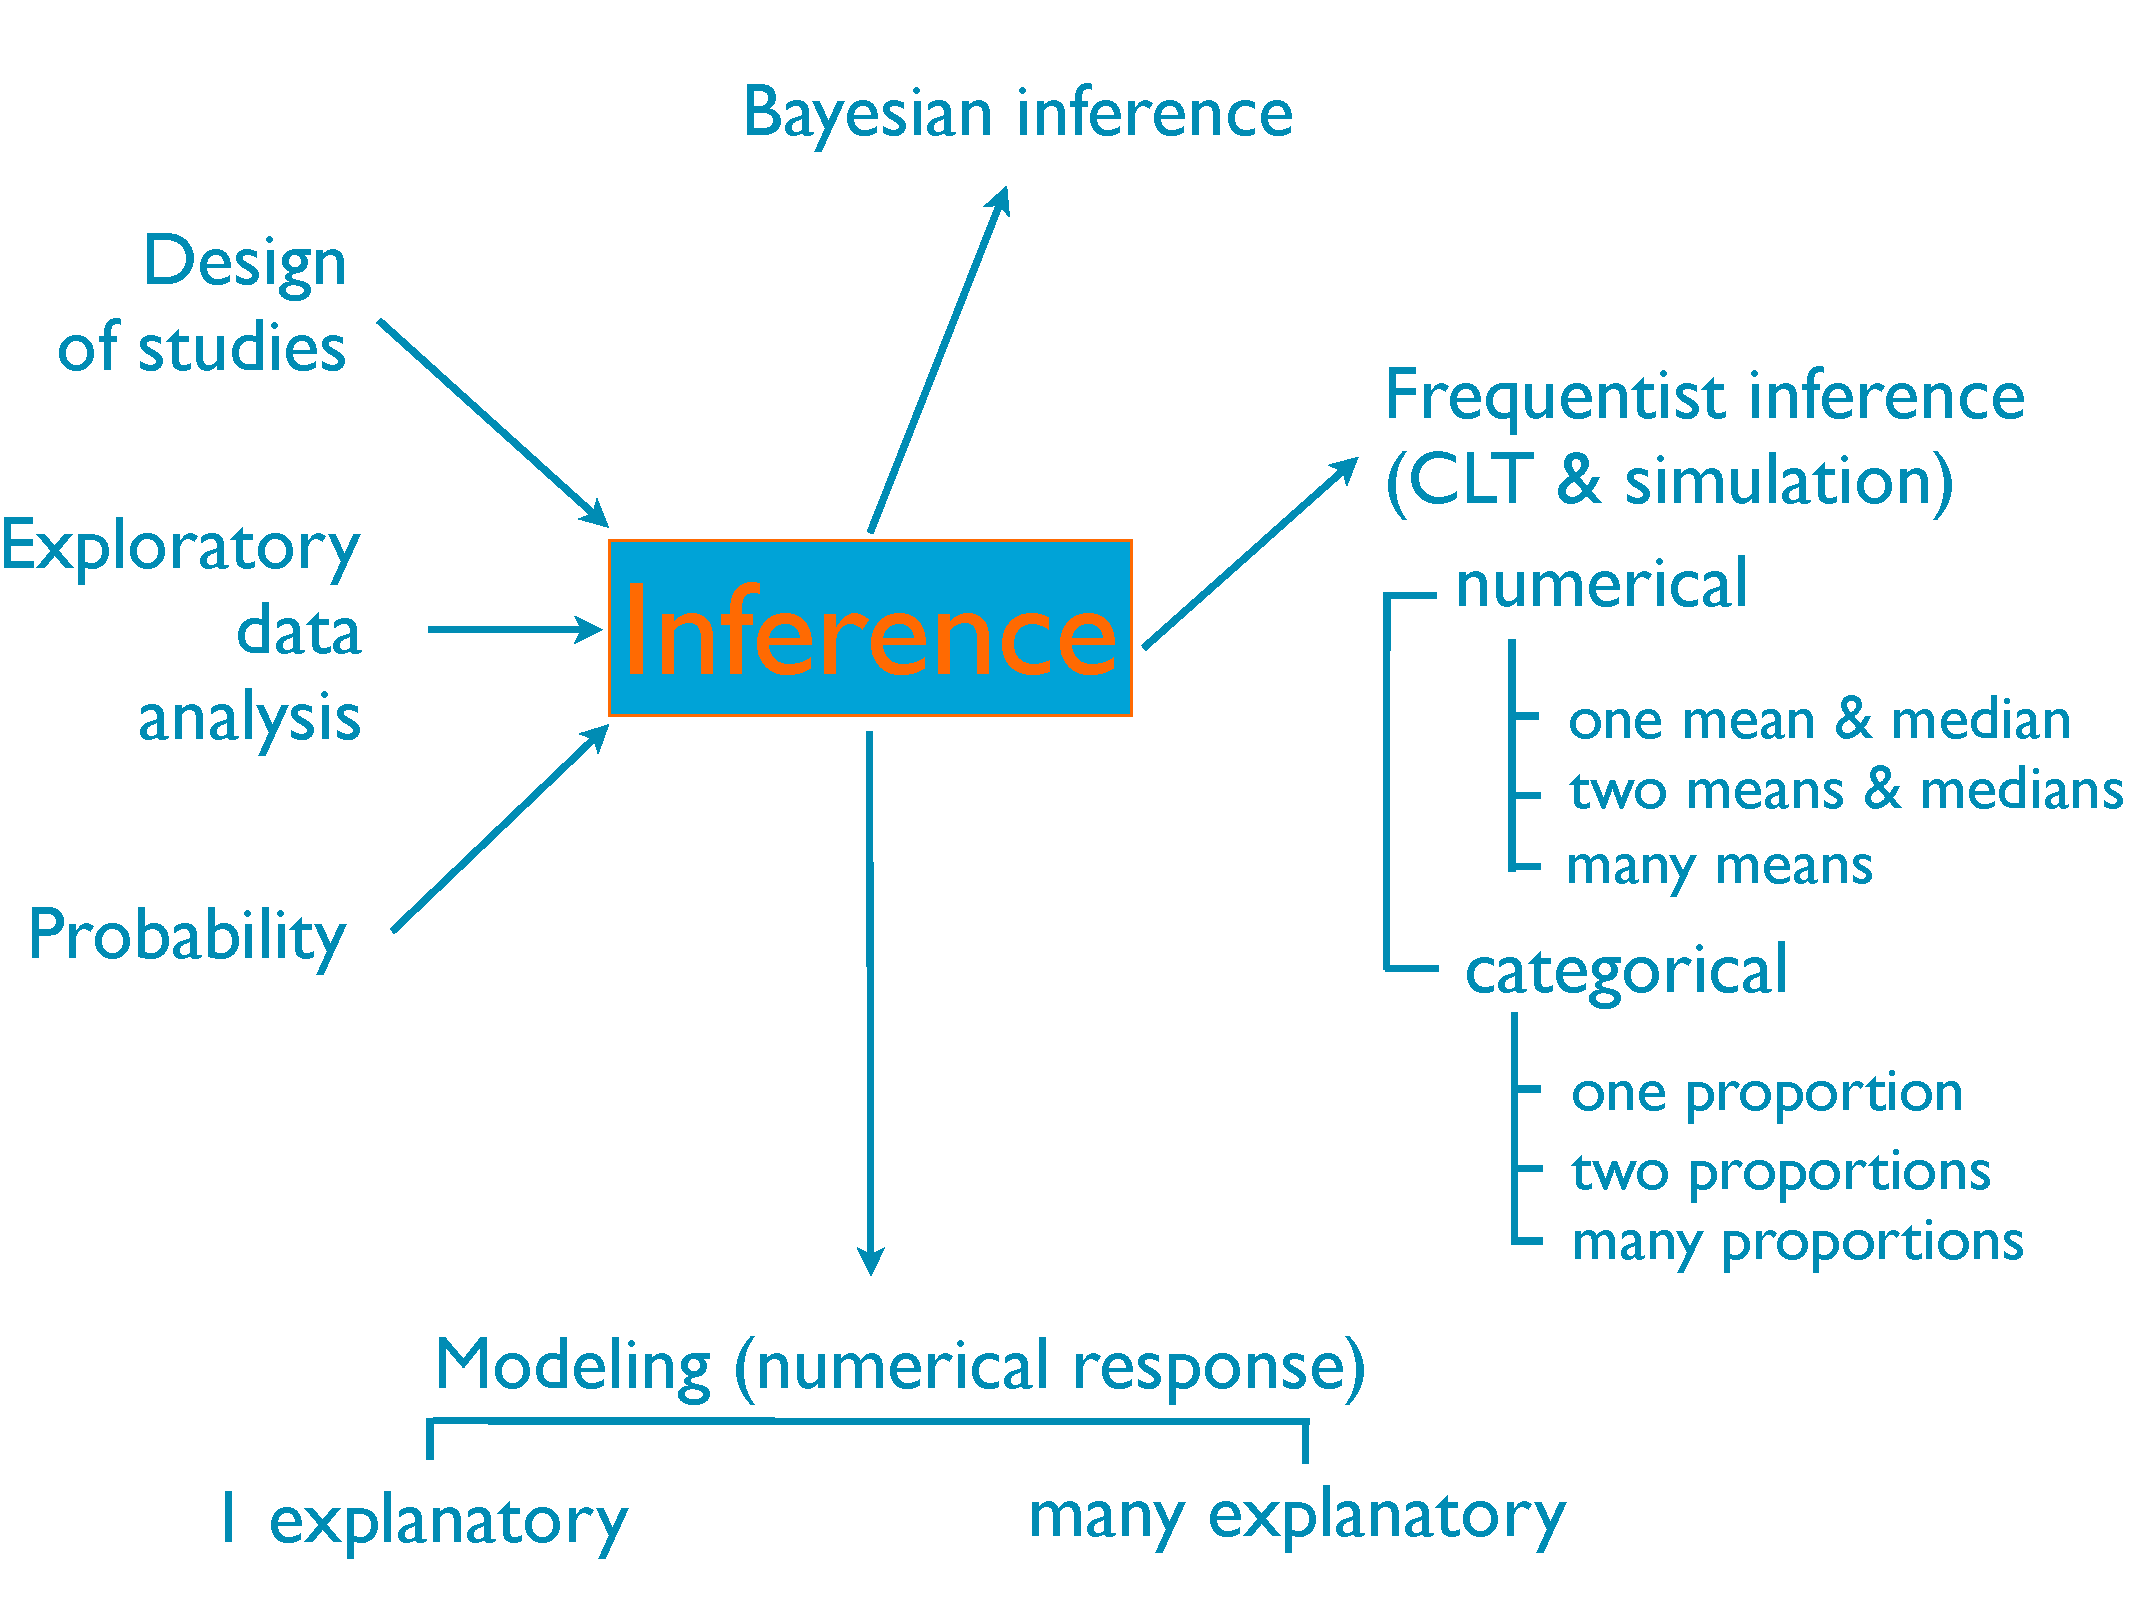
\includegraphics[width=\textwidth]{figures/map/inference}
}

\begin{enumerate}[(a)]
\item z-test
\item chi-square test of goodness of fit
\item \solnMult{anova}
\item \solnMult{linear regression}
\item t-test
\end{enumerate}

\end{frame}

%%%%%%%%%%%%%%%%%%%%%%%%%%%%%%%%%%%%

\begin{frame}[shrink]
\frametitle{Example - Breast Cancer \& Age}

{\small
It is theorized that an important risk factor for breast cancer is age at first birth. An international study was set up to test this hypothesis. Breast-cancer cases were identified among women in selected hospitals in the United States, Greece, Yugoslavia, Brazil, Taiwan, and Japan. Controls were chosen from women of comparable age who were in the hospital at the same time as the cases but who did not have breast cancer. All women were asked about their age at first birth.\\
~\\
The set of women with at least one birth was arbitrarily divided into two categories: (1) women whose age at first birth was less than or equal to 29 years and (2) women whose age at first birth was greater than of equal to 30 years. The following results were found among women with at least one birth: 683 of 3220 women with breast cancer (case women) and 1498 of 10,245 women without breast cancer (control women) had an age at first birth greater than or equal to 30. How can we assess whether this difference is significant or simply due to chance?\\
}
\end{frame}

%%%%%%%%%%%%%%%%%%%%%%%%%%%%%%%%%%

\begin{frame}
\frametitle{Breast Cancer \& Age - set-up}
{\small
We are comparing two categorical variables (breast cancer status vs. age at first birth), this can be summarized by a contingency table.\\
\vspace{2mm}
\only<2->{We are given 683 of 3220 women with breast cancer (case women) and 1498 of 10,245 women without breast cancer (control women) had an age at first birth greater than 30.}

\begin{center}
\begin{tabular}{r|c|c|c}
         & Breast Cancer   & No Breast Cancer & Total           \\
         & (case)          & (Controls)       &                 \\
\hline
         &                 &                  &                 \\
$\le 29$ & \only<4->{2537} & \only<6->{8747}  & \only<7->{11284}\\
         &                 &                  &                 \\
\hline
         &                 &                  &                 \\
$\ge 30$ & \only<3->{683}  & \only<5->{1498}  & \only<7->{2181} \\
         &                 &                  &                 \\
\hline
         &                 &                  &                 \\
Total    & \only<3->{3220} & \only<5->{10245} & \only<7->{13465}\\
\end{tabular}
\end{center}
}
\end{frame}

%%%%%%%%%%%%%%%%%%%%%%%%%%%%%%%%%%

\begin{frame}
\frametitle{Breast Cancer \& Age - set-up}

\vspace{-3mm}

\[ n_{case} = 3220,~n_{ctrl} = 10245 \]

\begin{itemize}
\item cases: \pause 13465 women (hospital patients) with at least one child
\item variable(s): \pause (1) breast cancer status - categorical, (2) age at first birth - categorical
\item parameter of interest: \pause $p_{case} - p_{ctrl}$
\begin{itemize}
\item  Note: $p_{case} = P(age \ge 30|case)$ and $p_{ctrl} = P(age \ge 30|ctrl)$
\end{itemize}
\item test: \pause compare two population proportion of independent groups
\item hypotheses: \pause (two-tailed)
\begin{itemize}
\item[] $H_0: p_{case}  =  p_{ctrl}$
\item[] $H_A: p_{case} \ne p_{ctrl}$
\end{itemize}
\end{itemize}

\end{frame}

%%%%%%%%%%%%%%%%%%%%%%%%%%%%%%%%%%

\begin{frame}
\frametitle{Breast Cancer \& Age - point estimate}

\clicker{Which of the following is the correct point estimate for this HT?}

{\small
\begin{center}
\begin{tabular}{r|c|c|c}
         & BC  & No BC & Total           \\
         & (Case)          & (Controls)       &                 \\
\hline
$\le 29$ & {2537} & {8747}  & {11284}\\
$\ge 30$ & {683}  & {1498}  & {2181} \\
\hline
Total    &{3220} &{10245} & {13465}\\
\end{tabular}
\end{center}
}

\begin{multicols}{2}
\begin{enumerate}[(a)]
\item $\frac{683}{2181} - \frac{1498}{2181}$
\item $\frac{683}{13465} - \frac{1498}{13465}$
\item $\frac{2537}{11284} - \frac{683}{2181}$
\item \solnMult{ $\frac{683}{3220} - \frac{1498}{10245}$} \only<2|handout:0>{\red{= 0.066}}
\item $\frac{683}{2181} - \frac{683}{3220}$
\item[]
\end{enumerate}
\end{multicols}

\end{frame}

%%%%%%%%%%%%%%%%%%%%%%%%%%%%%%%%%%

\begin{frame}
\frametitle{Breast Cancer \& Age - standard error}

\twocol{0.5}{0.5}{
\clicker{Which of the following is the correct standard error for this HT?}
}
{
{\footnotesize
\begin{center}
\begin{tabular}{r|c|c|c}
         & BC  & No BC & Total           \\
         & (Case)          & (Controls)       &                 \\
\hline
$\le 29$ & {2537} & {8747}  & {11284}\\
$\ge 30$ & {683}  & {1498}  & {2181} \\
\hline
Total    &{3220} &{10245} & {13465}\\
\hline
$\hat{p}$ & 0.212	& 0.146	& 0.162 \\
\end{tabular}
\end{center}
}
}

{\small
\begin{enumerate}[(a)]
\item $ \sqrt{ \frac{0.212 \times (1-0.212)}{3220}} + \sqrt{ \frac{0.146 \times (1-0.146)}{10245} }$
\item $ \sqrt{ \frac{0.212 \times (1-0.212)}{3220} + \frac{0.146 \times (1-0.146)}{10245} }$
\item \solnMult{ $ \sqrt{ \frac{0.162 \times (1-0.162)}{3220} + \frac{0.162 \times (1-0.162)}{10245} }$ } \only<2|handout:0>{\red{= 0.0074}}
\item $ \sqrt{ \frac{0.212 \times (1-0.212)}{13465} + \frac{0.146 \times (1-0.146)}{13465} }$
\item $ \sqrt{ \frac{0.162 \times (1-0.162)}{13465} + \frac{0.162 \times (1-0.162)}{13465} }$
\end{enumerate}
}

\end{frame}

%%%%%%%%%%%%%%%%%%%%%%%%%%%%%%%%%

\begin{frame}
\frametitle{Breast Cancer \& Age - test statistic \& p-value}

\[ Z = \frac{\hat{p}_{case}-\hat{p}_{ctrl} - 0}{SE} = \frac{0.212 - 0.146}{0.0074} = 8.92 \]

\pause

\[ \text{p-value} = P(Z > 8.92)+P(Z<-8.92) \approx 0 \]

\end{frame}

%%%%%%%%%%%%%%%%%%%%%%%%%%%%%%%%%%

\begin{frame}
\frametitle{Breast Cancer \& Age - confidence interval}

\begin{itemize}

\item Confidence level: 98\%

\pause

\item Theoretical: Using a critical value based on the Z distr. ($z^\star$):
\begin{align*} 
\text{point estimate} &\pm ME \\
= \text{point estimate} &\pm z^\star \times SE
\end{align*}

\end{itemize}

\pause

For a confidence interval, 
\begin{align*}
SE &= \sqrt{\frac{\hat{p}_{case}(1-\hat{p}_{case})}{n_{case}} + \frac{\hat{p}_{ctrl}(1-\hat{p}_{ctrl})}{n_{ctrl}} } \\
   &= \sqrt{\frac{0.212(1-0.212)}{3220} + \frac{0.146(1-0.146)}{10245}} = 0.008 
\end{align*}
\pause

\begin{eqnarray*}
(0.212 - 0.146) \pm 2.33 \times 0.008 &\approx& 0.066 \pm 0.0186 \\
\pause
&=& (0.0474,~0.0846)
\end{eqnarray*}

\end{frame}

%%%%%%%%%%%%%%%%%%%%%%%%%%%%%%%%%%
\begin{frame}

\twocol{0.7}{0.3}
{
{\scriptsize
\clicker{$n = 30$ and $\hat{p} = 0.6$. Hypotheses: $H_0: p = 0.8; H_A: p < 0.8$. Which of the following is an appropriate method for calculating the p-value for this test?
}}}
{
 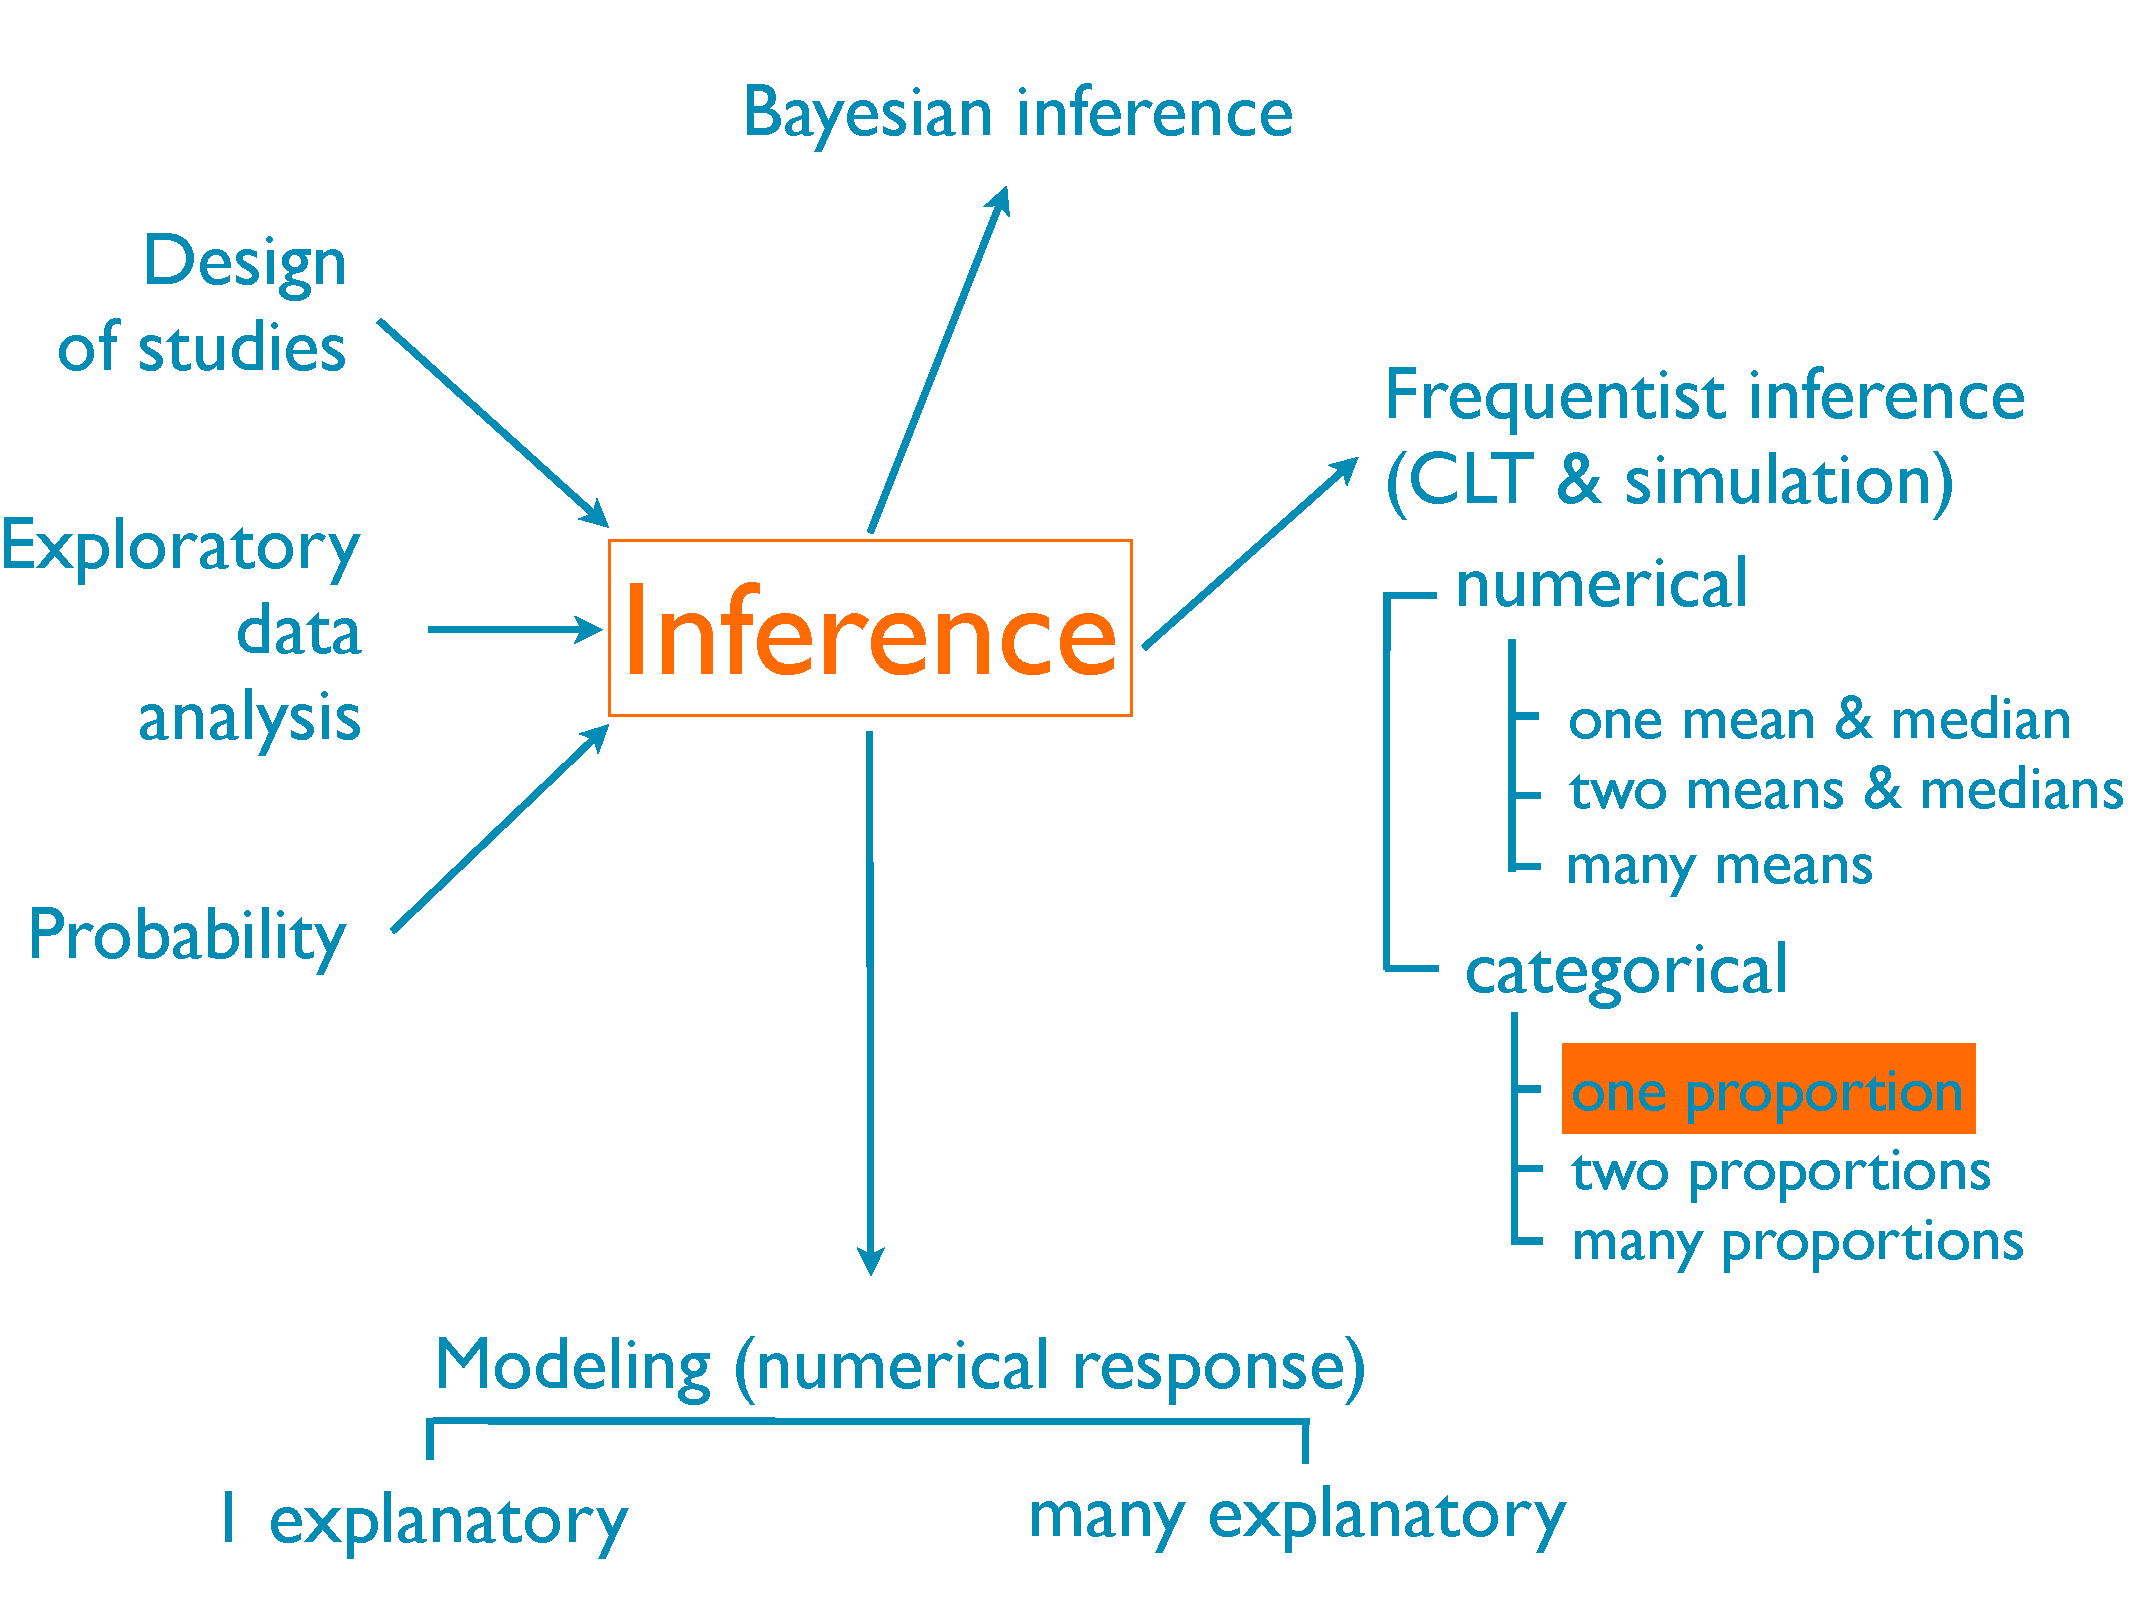
\includegraphics[width=\textwidth]{figures/map/one_prop}
}

\vfill

\begin{enumerate}[(a)]
\item \solnMult{CLT-based inference using the normal distribution}
\item simulation-based inference
\item \solnMult{exact calculation using the binomial distribution}
\end{enumerate}

\end{frame}

%%%%%%%%%%%%%%%%%%%%%%%%%%%%%%%%%%%%

\begin{frame}

\twocol{0.7}{0.3}
{
{\scriptsize
\clicker{$n = 30$ and $\hat{p} = 0.6$. Hypotheses: $H_0: p = 0.8; H_A: p < 0.8$. Suppose we wanted to use simulation-based methods. Which of the following is the correct set up for this hypothesis test? Red: success, blue: failure, $\hat{p}_{sim}$ = proportion of reds in simulated samples.
}}}
{
 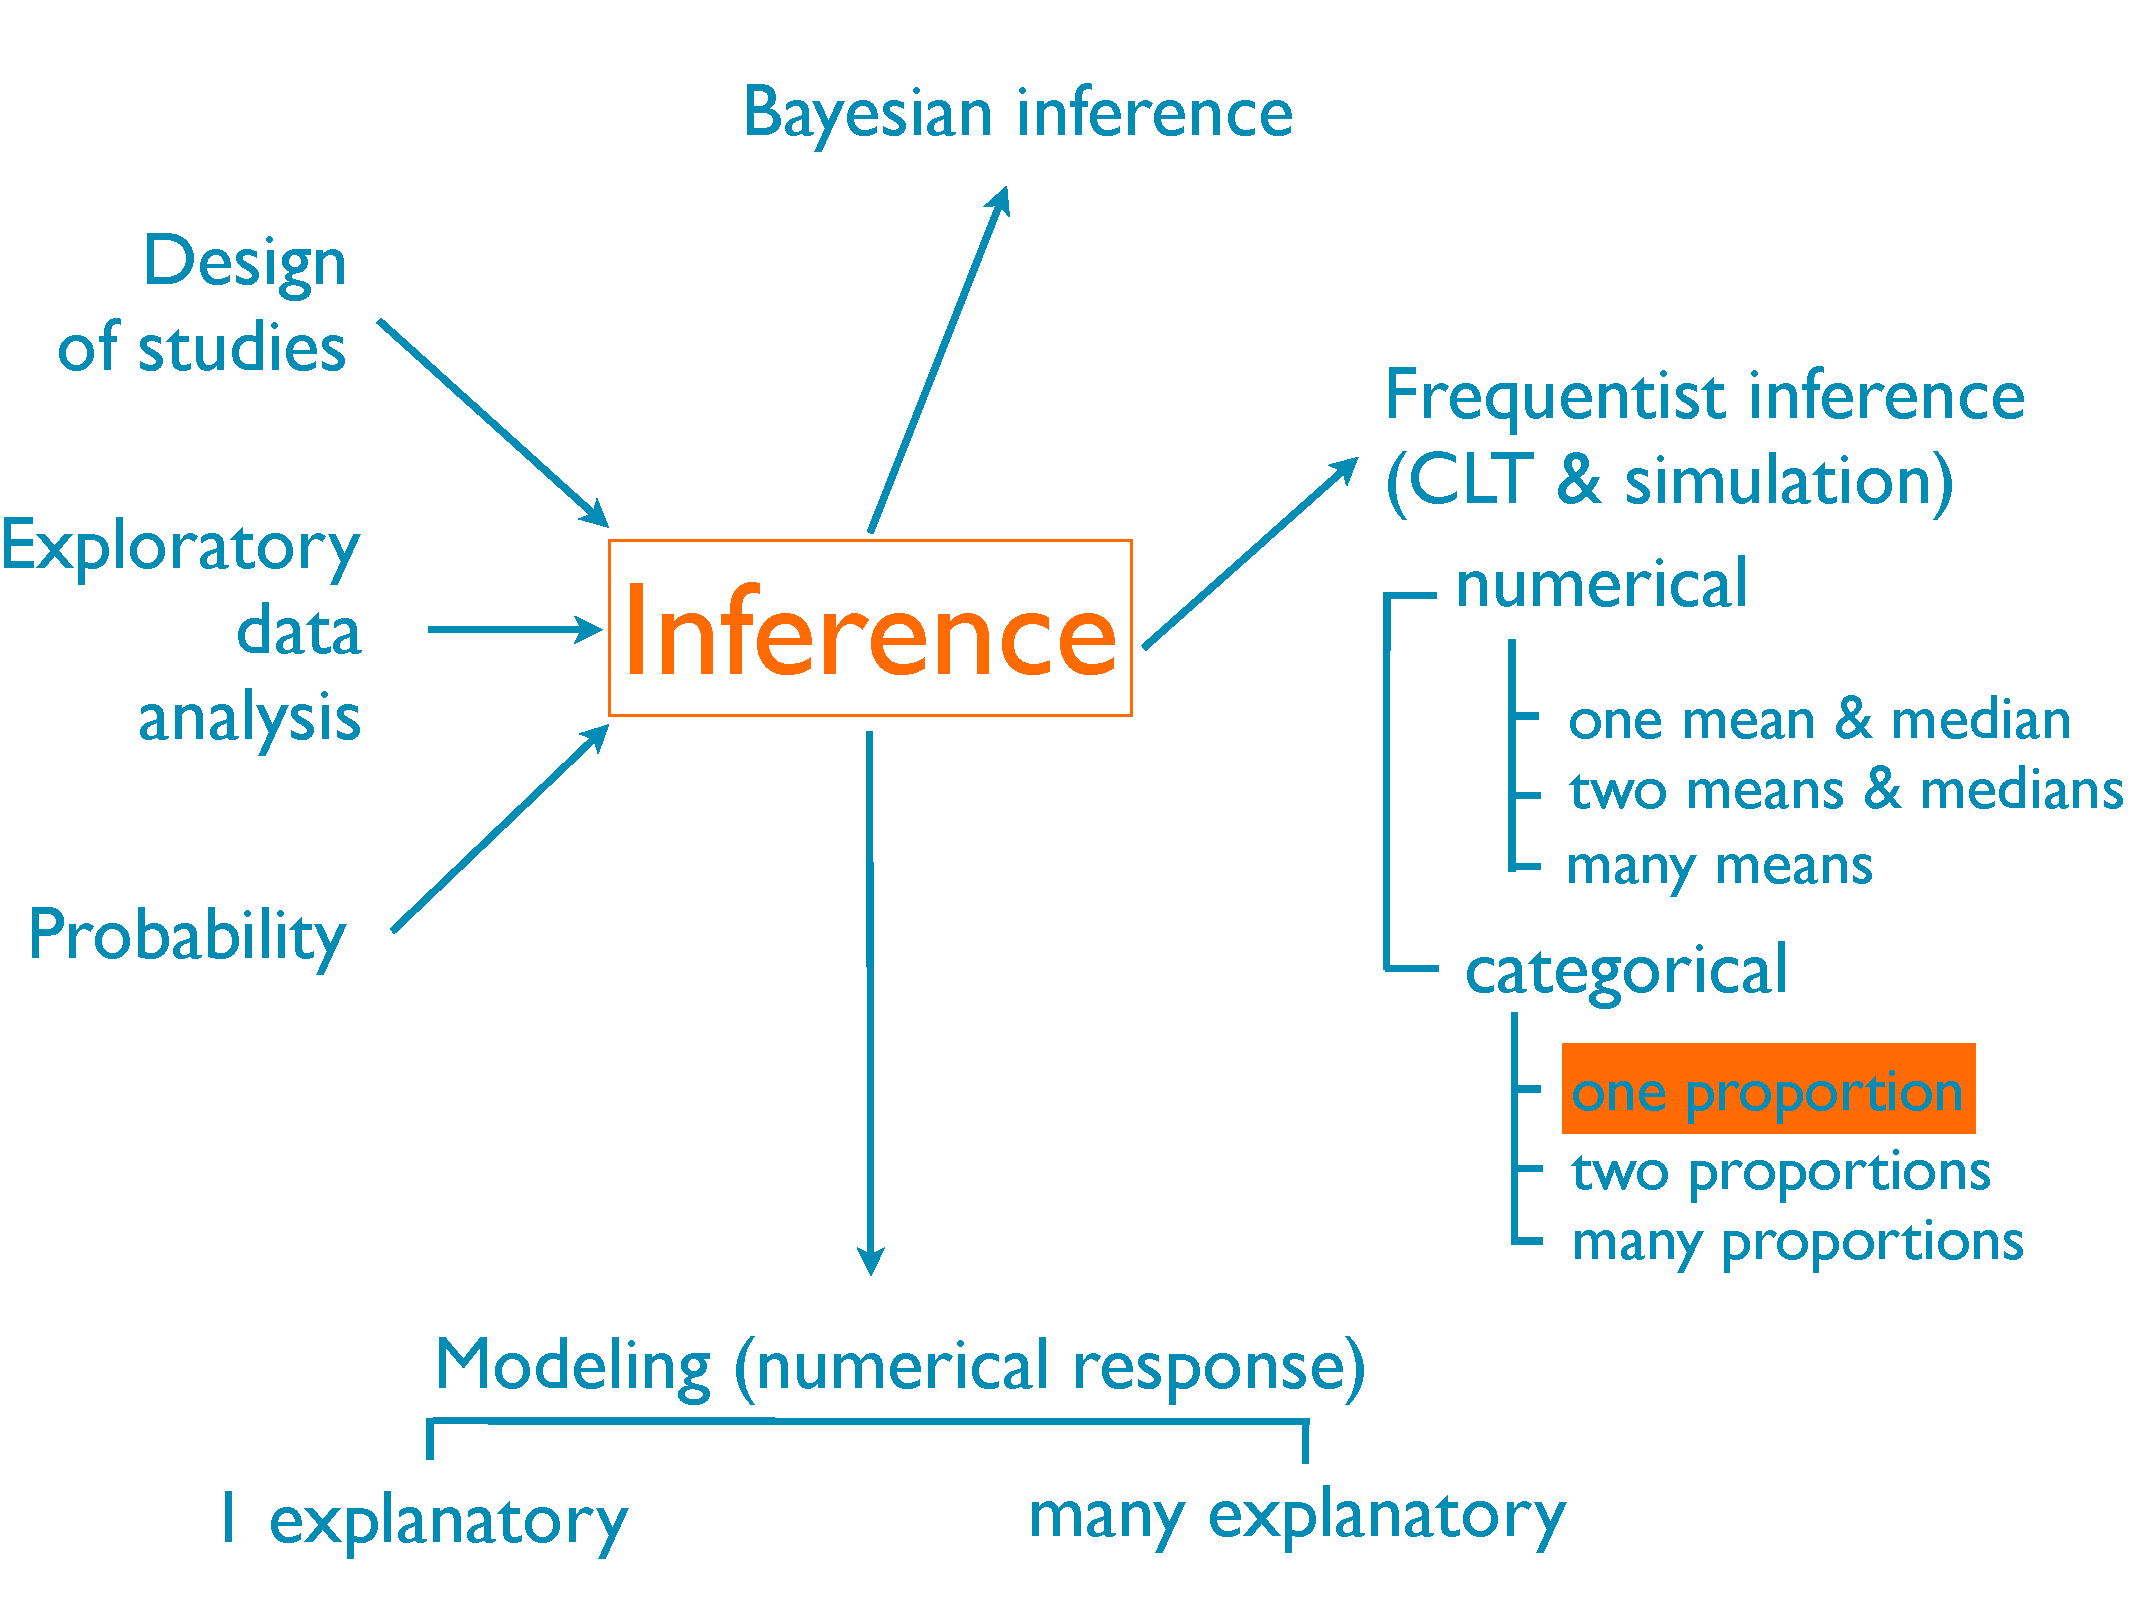
\includegraphics[width=\textwidth]{figures/map/one_prop}
}

\vfill

{\footnotesize
\begin{enumerate}[(a)]
\item Place 60 red and 40 blue chips in a bag. Sample, \underline{with} replacement, 30 chips and calculate the proportion of reds. Repeat this many times and calculate the proportion of simulations where $\hat{p}_{sim} \le 0.8$. 
\item Place 80 red and 20 blue chips in a bag. Sample, \underline{without} replacement, 30 chips and calculate the proportion of reds. Repeat this many times and calculate the proportion of simulations where $\hat{p}_{sim} \le 0.6$.
\item \solnMult{Place 80 red and 20 blue chips in a bag. Sample, \underline{with} replacement, 30 chips and calculate the proportion of reds. Repeat this many times and calculate the proportion of simulations where $\hat{p}_{sim} \le 0.6$.}
\item Place 80 red and 20 blue chips in a bag. Sample, \underline{with} replacement, 100 chips and calculate the proportion of reds. Repeat this many times and calculate the proportion of simulations where $\hat{p}_{sim} \le 0.6$. 
\end{enumerate}
}

\end{frame}

%%%%%%%%%%%%%%%%%%%%%%%%%%%%%%%%%%%

\end{document}